\documentclass[twoside]{book}

% Packages required by doxygen
\usepackage{calc}
\usepackage{doxygen}
\usepackage{graphicx}
\usepackage[utf8]{inputenc}
\usepackage{makeidx}
\usepackage{multicol}
\usepackage{multirow}
\usepackage{textcomp}
\usepackage[table]{xcolor}

% Font selection
\usepackage[T1]{fontenc}
\usepackage{mathptmx}
\usepackage[scaled=.90]{helvet}
\usepackage{courier}
\usepackage{amssymb}
\usepackage{sectsty}
\renewcommand{\familydefault}{\sfdefault}
\allsectionsfont{%
  \fontseries{bc}\selectfont%
  \color{darkgray}%
}
\renewcommand{\DoxyLabelFont}{%
  \fontseries{bc}\selectfont%
  \color{darkgray}%
}

% Page & text layout
\usepackage{geometry}
\geometry{%
  a4paper,%
  top=2.5cm,%
  bottom=2.5cm,%
  left=2.5cm,%
  right=2.5cm%
}
\tolerance=750
\hfuzz=15pt
\hbadness=750
\setlength{\emergencystretch}{15pt}
\setlength{\parindent}{0cm}
\setlength{\parskip}{0.2cm}
\makeatletter
\renewcommand{\paragraph}{%
  \@startsection{paragraph}{4}{0ex}{-1.0ex}{1.0ex}{%
    \normalfont\normalsize\bfseries\SS@parafont%
  }%
}
\renewcommand{\subparagraph}{%
  \@startsection{subparagraph}{5}{0ex}{-1.0ex}{1.0ex}{%
    \normalfont\normalsize\bfseries\SS@subparafont%
  }%
}
\makeatother

% Headers & footers
\usepackage{fancyhdr}
\pagestyle{fancyplain}
\fancyhead[LE]{\fancyplain{}{\bfseries\thepage}}
\fancyhead[CE]{\fancyplain{}{}}
\fancyhead[RE]{\fancyplain{}{\bfseries\leftmark}}
\fancyhead[LO]{\fancyplain{}{\bfseries\rightmark}}
\fancyhead[CO]{\fancyplain{}{}}
\fancyhead[RO]{\fancyplain{}{\bfseries\thepage}}
\fancyfoot[LE]{\fancyplain{}{}}
\fancyfoot[CE]{\fancyplain{}{}}
\fancyfoot[RE]{\fancyplain{}{\bfseries\scriptsize Generated on Mon Mar 9 2015 12\-:22\-:44 for Robot Simulator by Doxygen }}
\fancyfoot[LO]{\fancyplain{}{\bfseries\scriptsize Generated on Mon Mar 9 2015 12\-:22\-:44 for Robot Simulator by Doxygen }}
\fancyfoot[CO]{\fancyplain{}{}}
\fancyfoot[RO]{\fancyplain{}{}}
\renewcommand{\footrulewidth}{0.4pt}
\renewcommand{\chaptermark}[1]{%
  \markboth{#1}{}%
}
\renewcommand{\sectionmark}[1]{%
  \markright{\thesection\ #1}%
}

% Indices & bibliography
\usepackage{natbib}
\usepackage[titles]{tocloft}
\setcounter{tocdepth}{3}
\setcounter{secnumdepth}{5}
\makeindex

% Hyperlinks (required, but should be loaded last)
\usepackage{ifpdf}
\ifpdf
  \usepackage[pdftex,pagebackref=true]{hyperref}
\else
  \usepackage[ps2pdf,pagebackref=true]{hyperref}
\fi
\hypersetup{%
  colorlinks=true,%
  linkcolor=blue,%
  citecolor=blue,%
  unicode%
}

% Custom commands
\newcommand{\clearemptydoublepage}{%
  \newpage{\pagestyle{empty}\cleardoublepage}%
}


%===== C O N T E N T S =====

\begin{document}

% Titlepage & ToC
\hypersetup{pageanchor=false}
\pagenumbering{roman}
\begin{titlepage}
\vspace*{7cm}
\begin{center}%
{\Large Robot Simulator }\\
\vspace*{1cm}
{\large Generated by Doxygen 1.8.6}\\
\vspace*{0.5cm}
{\small Mon Mar 9 2015 12:22:44}\\
\end{center}
\end{titlepage}
\clearemptydoublepage
\tableofcontents
\clearemptydoublepage
\pagenumbering{arabic}
\hypersetup{pageanchor=true}

%--- Begin generated contents ---
\chapter{Robot Simulator Main Page}
\label{index}\hypertarget{index}{}\hypertarget{index_intro_sec}{}\section{Introduction}\label{index_intro_sec}
As an invaluable means to practice the concepts we are learning in class, we are engaging in a semester long software development project in which we are building a robot simulator. We are using the Iterative Method. This means that software requirements are being given to us in stages. Each stage (iteration) builds on the previous one by increasing its functionality and possibly modifying some of the previous requirements.

Our assignment is to construct a program that meets the functional requirements and demonstrates good software development practices. \char`\"{}\-Good\char`\"{} means clear, concise, thoughtful, and readable code that is well documented and thoroughly tested. The quality of our software is equally, if not more important, than its functionality. In this situation, we are quite confident that by utilizing good development practices, good functionality will naturally follow.

We are writing the simulator using C++ and the Open\-G\-L, G\-L\-U\-T, and G\-L\-U\-I Utility graphics environments. (The graphics are as simplistic as they can be.) We have already started to use these libraries in the labs, and, in addition to the many on-\/line resources, we will continue to receive instruction in labs and in lectures. Open\-G\-L, G\-L\-U\-T, and G\-L\-U\-I operate on any and all platforms. We must ensure this software works on C\-S\-E machines.\hypertarget{index_Execution}{}\section{Execution}\label{index_Execution}
To run the robot simulator, execute the following commands\-:


\begin{DoxyCode}
make clean
make all
./gorobot
\end{DoxyCode}


To run the test cases, execute the following commands\-:


\begin{DoxyCode}
make clean
make all
./testrobot
\end{DoxyCode}
 
\chapter{Namespace Index}
\section{Namespace List}
Here is a list of all documented namespaces with brief descriptions\-:\begin{DoxyCompactList}
\item\contentsline{section}{\hyperlink{namespaceDrawing}{Drawing} \\*A place to hold the render function }{\pageref{namespaceDrawing}}{}
\end{DoxyCompactList}

\chapter{Hierarchical Index}
\section{Class Hierarchy}
This inheritance list is sorted roughly, but not completely, alphabetically\-:\begin{DoxyCompactList}
\item \contentsline{section}{Base\-Gfx\-App}{\pageref{classBaseGfxApp}}{}
\begin{DoxyCompactList}
\item \contentsline{section}{Simulation}{\pageref{classSimulation}}{}
\end{DoxyCompactList}
\item \contentsline{section}{Clock}{\pageref{classClock}}{}
\item \contentsline{section}{Color}{\pageref{classColor}}{}
\item \contentsline{section}{Entity}{\pageref{classEntity}}{}
\begin{DoxyCompactList}
\item \contentsline{section}{Obstacle}{\pageref{classObstacle}}{}
\item \contentsline{section}{Robot\-Class}{\pageref{classRobotClass}}{}
\item \contentsline{section}{Target}{\pageref{classTarget}}{}
\end{DoxyCompactList}
\item \contentsline{section}{Entity\-Manager}{\pageref{classEntityManager}}{}
\item Test\-Suite\begin{DoxyCompactList}
\item \contentsline{section}{Entity\-Tests}{\pageref{classEntityTests}}{}
\end{DoxyCompactList}
\item \contentsline{section}{Vector2$<$ T $>$}{\pageref{classVector2}}{}
\item \contentsline{section}{Vector2$<$ float $>$}{\pageref{classVector2}}{}
\end{DoxyCompactList}

\chapter{Class Index}
\section{Class List}
Here are the classes, structs, unions and interfaces with brief descriptions\-:\begin{DoxyCompactList}
\item\contentsline{section}{\hyperlink{classBaseGfxApp}{Base\-Gfx\-App} }{\pageref{classBaseGfxApp}}{}
\item\contentsline{section}{\hyperlink{classClock}{Clock} }{\pageref{classClock}}{}
\item\contentsline{section}{\hyperlink{classColor}{Color} \\*A Three float holder for colors to be cast as (R,G,B) }{\pageref{classColor}}{}
\item\contentsline{section}{\hyperlink{classEntity}{Entity} \\*This is the base class for all Entities. Robots, targets, and obstacles are all derived from this class }{\pageref{classEntity}}{}
\item\contentsline{section}{\hyperlink{classEntityManager}{Entity\-Manager} \\*This class is used to manage entities }{\pageref{classEntityManager}}{}
\item\contentsline{section}{\hyperlink{classEntityTests}{Entity\-Tests} }{\pageref{classEntityTests}}{}
\item\contentsline{section}{\hyperlink{classObstacle}{Obstacle} \\*The class for creating obstacles }{\pageref{classObstacle}}{}
\item\contentsline{section}{\hyperlink{classRobotClass}{Robot\-Class} \\*The class for creating robots }{\pageref{classRobotClass}}{}
\item\contentsline{section}{\hyperlink{classSimulation}{Simulation} \\*Main application class for the robot simulation }{\pageref{classSimulation}}{}
\item\contentsline{section}{\hyperlink{classTarget}{Target} \\*The class for creating targets }{\pageref{classTarget}}{}
\item\contentsline{section}{\hyperlink{classVector2}{Vector2$<$ T $>$} \\*A two dimensional templated vector of the form (x, y) }{\pageref{classVector2}}{}
\end{DoxyCompactList}

\chapter{File Index}
\section{File List}
Here is a list of all documented files with brief descriptions\-:\begin{DoxyCompactList}
\item\contentsline{section}{\hyperlink{BaseGfxApp_8h}{Base\-Gfx\-App.\-h} \\*The basic application class for C\-Sci-\/3081 project. Uses G\-L\-U\-T and G\-L\-U\-I and wraps them in a nice C++ interface }{\pageref{BaseGfxApp_8h}}{}
\item\contentsline{section}{{\bfseries Clock.\-h} }{\pageref{Clock_8h}}{}
\item\contentsline{section}{{\bfseries Color.\-h} }{\pageref{Color_8h}}{}
\item\contentsline{section}{{\bfseries Drawing.\-h} }{\pageref{Drawing_8h}}{}
\item\contentsline{section}{{\bfseries Entity\-Tests.\-h} }{\pageref{EntityTests_8h}}{}
\item\contentsline{section}{\hyperlink{main_8cpp}{main.\-cpp} \\*Main function }{\pageref{main_8cpp}}{}
\item\contentsline{section}{{\bfseries mainpage.\-h} }{\pageref{mainpage_8h}}{}
\item\contentsline{section}{{\bfseries randf.\-h} }{\pageref{randf_8h}}{}
\item\contentsline{section}{{\bfseries Simulation.\-h} }{\pageref{Simulation_8h}}{}
\item\contentsline{section}{{\bfseries Vector2.\-h} }{\pageref{Vector2_8h}}{}
\item\contentsline{section}{Entity/{\bfseries Entity.\-h} }{\pageref{Entity_8h}}{}
\item\contentsline{section}{Entity/{\bfseries Entity\-Manager.\-h} }{\pageref{EntityManager_8h}}{}
\item\contentsline{section}{Entity/{\bfseries Obstacle.\-h} }{\pageref{Obstacle_8h}}{}
\item\contentsline{section}{Entity/{\bfseries Robot\-Class.\-h} }{\pageref{RobotClass_8h}}{}
\item\contentsline{section}{Entity/{\bfseries Target.\-h} }{\pageref{Target_8h}}{}
\end{DoxyCompactList}

\chapter{Namespace Documentation}
\hypertarget{namespaceDrawing}{\section{Drawing Namespace Reference}
\label{namespaceDrawing}\index{Drawing@{Drawing}}
}


A place to hold the render function.  


\subsection*{Functions}
\begin{DoxyCompactItemize}
\item 
void \hyperlink{namespaceDrawing_a18600f6b38e0e9fd5ca4d14d2c6c65f8}{draw\-Circle} (\hyperlink{classVector2}{Vector2f} position, float radius, \hyperlink{classColor}{Color} color)
\item 
void \hyperlink{namespaceDrawing_abf48d4f58682687283db03dd4af75c50}{draw\-Line} (\hyperlink{classVector2}{Vector2f} start, \hyperlink{classVector2}{Vector2f} end, \hyperlink{classColor}{Color} color, float line\-Width=4)
\item 
int \hyperlink{namespaceDrawing_aad23f577b63b549618750ebdad254ad3}{get\-Window\-Width} ()
\item 
int \hyperlink{namespaceDrawing_ae71c3e98ec705d2fc14f87c41f082324}{get\-Window\-Height} ()
\end{DoxyCompactItemize}


\subsection{Detailed Description}
A place to hold the render function. \begin{DoxyAuthor}{Author}
David Tran
\end{DoxyAuthor}
This namespace holds the drawing functions for rendering the entities. 

\subsection{Function Documentation}
\hypertarget{namespaceDrawing_a18600f6b38e0e9fd5ca4d14d2c6c65f8}{\index{Drawing@{Drawing}!draw\-Circle@{draw\-Circle}}
\index{draw\-Circle@{draw\-Circle}!Drawing@{Drawing}}
\subsubsection[{draw\-Circle}]{\setlength{\rightskip}{0pt plus 5cm}void Drawing\-::draw\-Circle (
\begin{DoxyParamCaption}
\item[{{\bf Vector2f}}]{position, }
\item[{float}]{radius, }
\item[{{\bf Color}}]{color}
\end{DoxyParamCaption}
)}}\label{namespaceDrawing_a18600f6b38e0e9fd5ca4d14d2c6c65f8}
Draw a circle 
\begin{DoxyParams}{Parameters}
{\em position} & the position of the circle in pixels (Vector2f) \\
\hline
{\em radius} & the radius of the circle in pixels (float) \\
\hline
{\em color} & the color of the circle (\hyperlink{classColor}{Color}) \\
\hline
\end{DoxyParams}
\hypertarget{namespaceDrawing_abf48d4f58682687283db03dd4af75c50}{\index{Drawing@{Drawing}!draw\-Line@{draw\-Line}}
\index{draw\-Line@{draw\-Line}!Drawing@{Drawing}}
\subsubsection[{draw\-Line}]{\setlength{\rightskip}{0pt plus 5cm}void Drawing\-::draw\-Line (
\begin{DoxyParamCaption}
\item[{{\bf Vector2f}}]{start, }
\item[{{\bf Vector2f}}]{end, }
\item[{{\bf Color}}]{color, }
\item[{float}]{line\-Width}
\end{DoxyParamCaption}
)}}\label{namespaceDrawing_abf48d4f58682687283db03dd4af75c50}
Draw a line 
\begin{DoxyParams}{Parameters}
{\em start} & the beginning point of the line (Vector2f) \\
\hline
{\em end} & the ending point of the line (Vector2f) \\
\hline
{\em color} & the color of the line (\hyperlink{classColor}{Color}) \\
\hline
{\em line\-Width} & (optional) the width of the line (float) \\
\hline
\end{DoxyParams}
\hypertarget{namespaceDrawing_ae71c3e98ec705d2fc14f87c41f082324}{\index{Drawing@{Drawing}!get\-Window\-Height@{get\-Window\-Height}}
\index{get\-Window\-Height@{get\-Window\-Height}!Drawing@{Drawing}}
\subsubsection[{get\-Window\-Height}]{\setlength{\rightskip}{0pt plus 5cm}int Drawing\-::get\-Window\-Height (
\begin{DoxyParamCaption}
{}
\end{DoxyParamCaption}
)}}\label{namespaceDrawing_ae71c3e98ec705d2fc14f87c41f082324}
Get the window height \begin{DoxyReturn}{Returns}
The window height (int) 
\end{DoxyReturn}
\hypertarget{namespaceDrawing_aad23f577b63b549618750ebdad254ad3}{\index{Drawing@{Drawing}!get\-Window\-Width@{get\-Window\-Width}}
\index{get\-Window\-Width@{get\-Window\-Width}!Drawing@{Drawing}}
\subsubsection[{get\-Window\-Width}]{\setlength{\rightskip}{0pt plus 5cm}int Drawing\-::get\-Window\-Width (
\begin{DoxyParamCaption}
{}
\end{DoxyParamCaption}
)}}\label{namespaceDrawing_aad23f577b63b549618750ebdad254ad3}
Get the window width \begin{DoxyReturn}{Returns}
The window width (int) 
\end{DoxyReturn}

\chapter{Class Documentation}
\hypertarget{classBaseGfxApp}{\section{Base\-Gfx\-App Class Reference}
\label{classBaseGfxApp}\index{Base\-Gfx\-App@{Base\-Gfx\-App}}
}
Inheritance diagram for Base\-Gfx\-App\-:\begin{figure}[H]
\begin{center}
\leavevmode
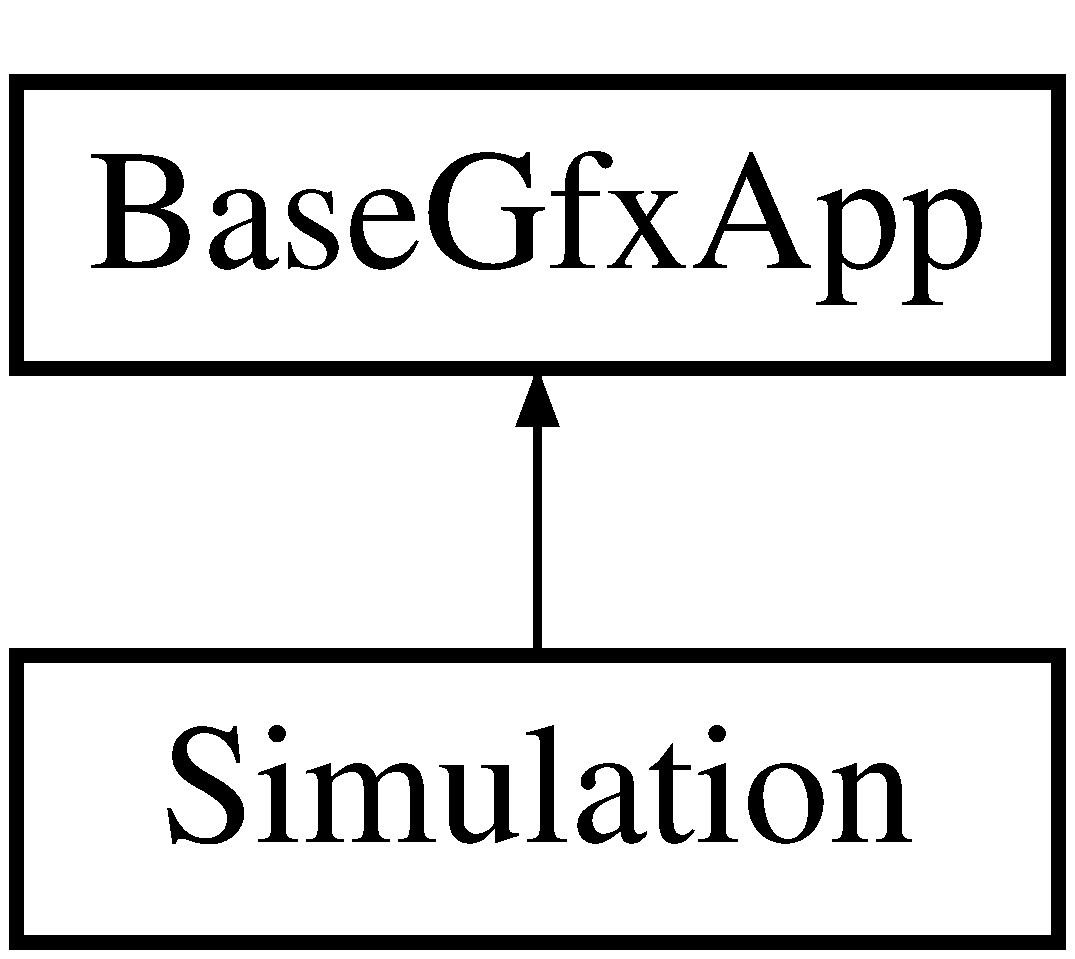
\includegraphics[height=2.000000cm]{classBaseGfxApp}
\end{center}
\end{figure}
\subsection*{Public Member Functions}
\begin{DoxyCompactItemize}
\item 
\hypertarget{classBaseGfxApp_a534a4b5293a35947fdae3805a103541d}{{\bfseries Base\-Gfx\-App} (int argc, char $\ast$argv\mbox{[}$\,$\mbox{]}, int width, int height, int x, int y, int glut\-Flags, bool create\-G\-L\-U\-I\-Win, int glui\-Win\-X, int glui\-Win\-Y)}\label{classBaseGfxApp_a534a4b5293a35947fdae3805a103541d}

\item 
\hypertarget{classBaseGfxApp_a4b3b1a475b7f2babaf1b477c34b15fb1}{void {\bfseries set\-Caption} (const std\-::string \&caption)}\label{classBaseGfxApp_a4b3b1a475b7f2babaf1b477c34b15fb1}

\item 
\hypertarget{classBaseGfxApp_acda031916c00d56c2dc901e2653e3083}{void {\bfseries run\-Main\-Loop} ()}\label{classBaseGfxApp_acda031916c00d56c2dc901e2653e3083}

\item 
\hypertarget{classBaseGfxApp_a35b64aa3d604736ceb036698d1a0b2d0}{virtual void {\bfseries update} ()}\label{classBaseGfxApp_a35b64aa3d604736ceb036698d1a0b2d0}

\item 
\hypertarget{classBaseGfxApp_ac8de2d5a955582547af5619b771b4d6d}{virtual void {\bfseries display} ()}\label{classBaseGfxApp_ac8de2d5a955582547af5619b771b4d6d}

\item 
\hypertarget{classBaseGfxApp_a0956b82d7fa58b623c498aea7073dbba}{virtual void {\bfseries mouse\-Moved} (int x, int y)}\label{classBaseGfxApp_a0956b82d7fa58b623c498aea7073dbba}

\item 
\hypertarget{classBaseGfxApp_abb23f716dd6612b3a72938e41525d338}{virtual void {\bfseries mouse\-Dragged} (int x, int y)}\label{classBaseGfxApp_abb23f716dd6612b3a72938e41525d338}

\item 
\hypertarget{classBaseGfxApp_aaaccf5a5e923a9465441a5ee712424a8}{virtual void {\bfseries left\-Mouse\-Down} (int x, int y)}\label{classBaseGfxApp_aaaccf5a5e923a9465441a5ee712424a8}

\item 
\hypertarget{classBaseGfxApp_a0a2961a932b02b2f9d7d0bb408f6fb51}{virtual void {\bfseries left\-Mouse\-Up} (int x, int y)}\label{classBaseGfxApp_a0a2961a932b02b2f9d7d0bb408f6fb51}

\item 
\hypertarget{classBaseGfxApp_afa87e6a71220945e41f0424e540125d9}{virtual void {\bfseries right\-Mouse\-Down} (int x, int y)}\label{classBaseGfxApp_afa87e6a71220945e41f0424e540125d9}

\item 
\hypertarget{classBaseGfxApp_a812643d563522a993457dd565c33f8f6}{virtual void {\bfseries right\-Mouse\-Up} (int x, int y)}\label{classBaseGfxApp_a812643d563522a993457dd565c33f8f6}

\item 
\hypertarget{classBaseGfxApp_a2c98cae9bb5ad1fb1832a6d4812670f8}{virtual void {\bfseries middle\-Mouse\-Down} (int x, int y)}\label{classBaseGfxApp_a2c98cae9bb5ad1fb1832a6d4812670f8}

\item 
\hypertarget{classBaseGfxApp_a00fc05e8d9629b72302b5adf014bdb0c}{virtual void {\bfseries middle\-Mouse\-Up} (int x, int y)}\label{classBaseGfxApp_a00fc05e8d9629b72302b5adf014bdb0c}

\item 
\hypertarget{classBaseGfxApp_a6d91e0cb7a3d48cad33956efe7eb36ca}{virtual void {\bfseries keyboard} (unsigned char c, int x, int y)}\label{classBaseGfxApp_a6d91e0cb7a3d48cad33956efe7eb36ca}

\item 
\hypertarget{classBaseGfxApp_a345566e62c9e4ec3705ec4d1c4c75f1f}{virtual void {\bfseries keyboard\-Special} (int key, int x, int y)}\label{classBaseGfxApp_a345566e62c9e4ec3705ec4d1c4c75f1f}

\item 
\hypertarget{classBaseGfxApp_acc4a40ce11edd6b6660a19cb4802a2bf}{virtual void {\bfseries keyboard\-Up} (unsigned char c, int x, int y)}\label{classBaseGfxApp_acc4a40ce11edd6b6660a19cb4802a2bf}

\item 
\hypertarget{classBaseGfxApp_afd14b435ff93b1e7f461cb8bd1a6fd59}{virtual void {\bfseries keyboard\-Special\-Up} (int key, int x, int y)}\label{classBaseGfxApp_afd14b435ff93b1e7f461cb8bd1a6fd59}

\item 
\hypertarget{classBaseGfxApp_a5d8d5d778a8aecd7f5f8e9c87f4c3d20}{virtual void {\bfseries reshape} (int width, int height)}\label{classBaseGfxApp_a5d8d5d778a8aecd7f5f8e9c87f4c3d20}

\item 
\hypertarget{classBaseGfxApp_a2978a7c358794c67df73b66776b2cef3}{virtual void {\bfseries glui\-Control} (int control\-I\-D)}\label{classBaseGfxApp_a2978a7c358794c67df73b66776b2cef3}

\item 
\hypertarget{classBaseGfxApp_ace089a1a94fb6bb0bc17e1b7fa48e05d}{int {\bfseries width} () const }\label{classBaseGfxApp_ace089a1a94fb6bb0bc17e1b7fa48e05d}

\item 
\hypertarget{classBaseGfxApp_aa253dbe16a20c40e0a1bf8ff942ceea3}{int {\bfseries height} () const }\label{classBaseGfxApp_aa253dbe16a20c40e0a1bf8ff942ceea3}

\item 
\hypertarget{classBaseGfxApp_ae9779f948eff6f45beec08091e98a803}{int {\bfseries handle} ()}\label{classBaseGfxApp_ae9779f948eff6f45beec08091e98a803}

\item 
\hypertarget{classBaseGfxApp_ac721a0fedce80308c5c0e5695016e95d}{G\-L\-U\-I $\ast$ {\bfseries glui} ()}\label{classBaseGfxApp_ac721a0fedce80308c5c0e5695016e95d}

\end{DoxyCompactItemize}
\subsection*{Static Protected Member Functions}
\begin{DoxyCompactItemize}
\item 
\hypertarget{classBaseGfxApp_a5fe6a77d37044cbe28647ed3391bbb7a}{static void {\bfseries s\-\_\-reshape} (int width, int height)}\label{classBaseGfxApp_a5fe6a77d37044cbe28647ed3391bbb7a}

\item 
\hypertarget{classBaseGfxApp_a52edb2569227319feb68779844e7d857}{static void {\bfseries s\-\_\-keyboard} (unsigned char c, int x, int y)}\label{classBaseGfxApp_a52edb2569227319feb68779844e7d857}

\item 
\hypertarget{classBaseGfxApp_a1e8d90a4faab60300ddf2a4ea9b83115}{static void {\bfseries s\-\_\-keyboardspecial} (int key, int x, int y)}\label{classBaseGfxApp_a1e8d90a4faab60300ddf2a4ea9b83115}

\item 
\hypertarget{classBaseGfxApp_aa1ca205af9d6cee33949f2e6adf4c923}{static void {\bfseries s\-\_\-keyboardup} (unsigned char c, int x, int y)}\label{classBaseGfxApp_aa1ca205af9d6cee33949f2e6adf4c923}

\item 
\hypertarget{classBaseGfxApp_a0e4dfe006f3cc9126c1cc8ad32784f75}{static void {\bfseries s\-\_\-keyboardspecialup} (int key, int x, int y)}\label{classBaseGfxApp_a0e4dfe006f3cc9126c1cc8ad32784f75}

\item 
\hypertarget{classBaseGfxApp_a5e640f2394f7e038d0dd2b469d5c2e24}{static void {\bfseries s\-\_\-mousemotion} (int x, int y)}\label{classBaseGfxApp_a5e640f2394f7e038d0dd2b469d5c2e24}

\item 
\hypertarget{classBaseGfxApp_a22dd953bfb75add9fd0f8f2f8be535c5}{static void {\bfseries s\-\_\-mousebtn} (int b, int s, int x, int y)}\label{classBaseGfxApp_a22dd953bfb75add9fd0f8f2f8be535c5}

\item 
\hypertarget{classBaseGfxApp_a38ab80de2e628af3093805b94858fc32}{static void {\bfseries s\-\_\-update} ()}\label{classBaseGfxApp_a38ab80de2e628af3093805b94858fc32}

\item 
\hypertarget{classBaseGfxApp_a58415c6151a2a80e1fe2eaa9919a4dab}{static void {\bfseries s\-\_\-draw} ()}\label{classBaseGfxApp_a58415c6151a2a80e1fe2eaa9919a4dab}

\item 
\hypertarget{classBaseGfxApp_ad4a963321f1147d68369225ab0c7f32f}{static void {\bfseries s\-\_\-gluicallback} (int control\-I\-D)}\label{classBaseGfxApp_ad4a963321f1147d68369225ab0c7f32f}

\end{DoxyCompactItemize}
\subsection*{Protected Attributes}
\begin{DoxyCompactItemize}
\item 
int \hyperlink{classBaseGfxApp_ad8697d6fdd10e6f336c3a662016b4fa7}{m\-\_\-glut\-Window\-Handle}
\item 
\hypertarget{classBaseGfxApp_a6eb1673b80283727221da2242211af1d}{G\-L\-U\-I $\ast$ {\bfseries m\-\_\-glui}}\label{classBaseGfxApp_a6eb1673b80283727221da2242211af1d}

\item 
\hypertarget{classBaseGfxApp_a2e70a389224f8affe7c137f7e20dc8c1}{bool {\bfseries m\-\_\-drag}}\label{classBaseGfxApp_a2e70a389224f8affe7c137f7e20dc8c1}

\item 
\hypertarget{classBaseGfxApp_a7e5ef1c8f25fe081b4a1fd4ce6a96e07}{int {\bfseries m\-\_\-width}}\label{classBaseGfxApp_a7e5ef1c8f25fe081b4a1fd4ce6a96e07}

\item 
\hypertarget{classBaseGfxApp_ac078e4fc20b5c2fe0c744966b850b412}{int {\bfseries m\-\_\-height}}\label{classBaseGfxApp_ac078e4fc20b5c2fe0c744966b850b412}

\end{DoxyCompactItemize}
\subsection*{Static Protected Attributes}
\begin{DoxyCompactItemize}
\item 
static \hyperlink{classBaseGfxApp}{Base\-Gfx\-App} $\ast$ \hyperlink{classBaseGfxApp_a65ba89b98af31e2649a0546631931000}{s\-\_\-current\-App} = N\-U\-L\-L
\item 
static bool \hyperlink{classBaseGfxApp_afa4690383ea27713016ef75b9fb1e42f}{s\-\_\-glut\-Initialized} = false
\end{DoxyCompactItemize}


\subsection{Member Data Documentation}
\hypertarget{classBaseGfxApp_ad8697d6fdd10e6f336c3a662016b4fa7}{\index{Base\-Gfx\-App@{Base\-Gfx\-App}!m\-\_\-glut\-Window\-Handle@{m\-\_\-glut\-Window\-Handle}}
\index{m\-\_\-glut\-Window\-Handle@{m\-\_\-glut\-Window\-Handle}!BaseGfxApp@{Base\-Gfx\-App}}
\subsubsection[{m\-\_\-glut\-Window\-Handle}]{\setlength{\rightskip}{0pt plus 5cm}int Base\-Gfx\-App\-::m\-\_\-glut\-Window\-Handle\hspace{0.3cm}{\ttfamily [protected]}}}\label{classBaseGfxApp_ad8697d6fdd10e6f336c3a662016b4fa7}
Underlying glut window handle \hypertarget{classBaseGfxApp_a65ba89b98af31e2649a0546631931000}{\index{Base\-Gfx\-App@{Base\-Gfx\-App}!s\-\_\-current\-App@{s\-\_\-current\-App}}
\index{s\-\_\-current\-App@{s\-\_\-current\-App}!BaseGfxApp@{Base\-Gfx\-App}}
\subsubsection[{s\-\_\-current\-App}]{\setlength{\rightskip}{0pt plus 5cm}{\bf Base\-Gfx\-App} $\ast$ Base\-Gfx\-App\-::s\-\_\-current\-App = N\-U\-L\-L\hspace{0.3cm}{\ttfamily [static]}, {\ttfamily [protected]}}}\label{classBaseGfxApp_a65ba89b98af31e2649a0546631931000}
G\-L\-U\-T and G\-L\-U\-I event callbacks are sent to the current window/app. Right now, there is only one window anyway (not counting the G\-L\-U\-I U\-I window.. in the future could be extended to support more windows. In any case, some structure like this is always needed when using glut with C++, since the glut callbacks must be either global or static functions. \hypertarget{classBaseGfxApp_afa4690383ea27713016ef75b9fb1e42f}{\index{Base\-Gfx\-App@{Base\-Gfx\-App}!s\-\_\-glut\-Initialized@{s\-\_\-glut\-Initialized}}
\index{s\-\_\-glut\-Initialized@{s\-\_\-glut\-Initialized}!BaseGfxApp@{Base\-Gfx\-App}}
\subsubsection[{s\-\_\-glut\-Initialized}]{\setlength{\rightskip}{0pt plus 5cm}bool Base\-Gfx\-App\-::s\-\_\-glut\-Initialized = false\hspace{0.3cm}{\ttfamily [static]}, {\ttfamily [protected]}}}\label{classBaseGfxApp_afa4690383ea27713016ef75b9fb1e42f}
Has glut\-Init been called? (only allowed once per program) 

The documentation for this class was generated from the following files\-:\begin{DoxyCompactItemize}
\item 
\hyperlink{BaseGfxApp_8h}{Base\-Gfx\-App.\-h}\item 
Base\-Gfx\-App.\-cpp\end{DoxyCompactItemize}

\hypertarget{classClock}{\section{Clock Class Reference}
\label{classClock}\index{Clock@{Clock}}
}


{\ttfamily \#include $<$Clock.\-h$>$}

\subsection*{Public Member Functions}
\begin{DoxyCompactItemize}
\item 
void \hyperlink{classClock_ae7c6708cf04b233655b501a97bb1e802}{update} ()
\item 
float \hyperlink{classClock_aa6bbd46f251a01c56f09ecfd89bcf324}{get\-Delta\-Time} ()
\item 
float \hyperlink{classClock_a7209991f330ee3d13557ac83ece52a5a}{get\-Current\-Time} ()
\end{DoxyCompactItemize}
\subsection*{Static Public Member Functions}
\begin{DoxyCompactItemize}
\item 
static \hyperlink{classClock}{Clock} \& \hyperlink{classClock_ab177004c1bc5df14899133b1e18c9bdb}{get\-Instance} ()
\end{DoxyCompactItemize}


\subsection{Detailed Description}
This class holds information about the time of the program 

\subsection{Member Function Documentation}
\hypertarget{classClock_a7209991f330ee3d13557ac83ece52a5a}{\index{Clock@{Clock}!get\-Current\-Time@{get\-Current\-Time}}
\index{get\-Current\-Time@{get\-Current\-Time}!Clock@{Clock}}
\subsubsection[{get\-Current\-Time}]{\setlength{\rightskip}{0pt plus 5cm}float Clock\-::get\-Current\-Time (
\begin{DoxyParamCaption}
{}
\end{DoxyParamCaption}
)}}\label{classClock_a7209991f330ee3d13557ac83ece52a5a}
Get the time since the program began \begin{DoxyReturn}{Returns}
time as seconds in a float 
\end{DoxyReturn}
\hypertarget{classClock_aa6bbd46f251a01c56f09ecfd89bcf324}{\index{Clock@{Clock}!get\-Delta\-Time@{get\-Delta\-Time}}
\index{get\-Delta\-Time@{get\-Delta\-Time}!Clock@{Clock}}
\subsubsection[{get\-Delta\-Time}]{\setlength{\rightskip}{0pt plus 5cm}float Clock\-::get\-Delta\-Time (
\begin{DoxyParamCaption}
{}
\end{DoxyParamCaption}
)}}\label{classClock_aa6bbd46f251a01c56f09ecfd89bcf324}
Get the time between frames \begin{DoxyReturn}{Returns}
delta time as seconds in a float 
\end{DoxyReturn}
\hypertarget{classClock_ab177004c1bc5df14899133b1e18c9bdb}{\index{Clock@{Clock}!get\-Instance@{get\-Instance}}
\index{get\-Instance@{get\-Instance}!Clock@{Clock}}
\subsubsection[{get\-Instance}]{\setlength{\rightskip}{0pt plus 5cm}{\bf Clock} \& Clock\-::get\-Instance (
\begin{DoxyParamCaption}
{}
\end{DoxyParamCaption}
)\hspace{0.3cm}{\ttfamily [static]}}}\label{classClock_ab177004c1bc5df14899133b1e18c9bdb}
Get the \hyperlink{classClock}{Clock} instance \begin{DoxyReturn}{Returns}
the instance of \hyperlink{classClock}{Clock} 
\end{DoxyReturn}
\hypertarget{classClock_ae7c6708cf04b233655b501a97bb1e802}{\index{Clock@{Clock}!update@{update}}
\index{update@{update}!Clock@{Clock}}
\subsubsection[{update}]{\setlength{\rightskip}{0pt plus 5cm}void Clock\-::update (
\begin{DoxyParamCaption}
{}
\end{DoxyParamCaption}
)}}\label{classClock_ae7c6708cf04b233655b501a97bb1e802}
Update the clock's time 

The documentation for this class was generated from the following files\-:\begin{DoxyCompactItemize}
\item 
Clock.\-h\item 
Clock.\-cpp\end{DoxyCompactItemize}

\hypertarget{classColor}{\section{Color Class Reference}
\label{classColor}\index{Color@{Color}}
}


A Three float holder for colors to be cast as (R,G,B)  




{\ttfamily \#include $<$Color.\-h$>$}

\subsection*{Public Member Functions}
\begin{DoxyCompactItemize}
\item 
\hyperlink{classColor_a9a742cbe9f9f4037f5d9f4e81a9b2428}{Color} ()
\item 
\hyperlink{classColor_af07af8fc1b1002d1d2db8f3d54ba28e9}{Color} (float input\-\_\-red, float input\-\_\-green, float input\-\_\-blue)
\item 
\hyperlink{classColor}{Color} \hyperlink{classColor_a268ca441e6c1780c77f5769d0713aede}{set\-Colors} (float input\-\_\-red, float input\-\_\-green, float input\-\_\-blue)
\item 
\hyperlink{classColor}{Color} \hyperlink{classColor_aacd0b5d30356e51a1b57151cbe49fd57}{set\-Red} (float input\-\_\-red)
\item 
\hyperlink{classColor}{Color} \hyperlink{classColor_a1892a99de7cca54543b4dc954413f7f6}{set\-Green} (float input\-\_\-green)
\item 
\hyperlink{classColor}{Color} \hyperlink{classColor_aa7fee41dde5551c88c68f91a7d5d15cb}{set\-Blue} (float input\-\_\-blue)
\item 
\hyperlink{classColor}{Color} \hyperlink{classColor_a2c287302d9a5f07a1dfd6b40f9ff10a4}{turn\-Red} ()
\item 
\hyperlink{classColor}{Color} \hyperlink{classColor_a2087acc41f2e0a62b907a91c31fe4d2d}{turn\-Green} ()
\item 
\hyperlink{classColor}{Color} \hyperlink{classColor_a27dedddac29c7915f3f2c1c262e903e3}{turn\-Blue} ()
\item 
\hyperlink{classColor}{Color} \hyperlink{classColor_a85f91c5e08f43ef23de5d757b9c39b80}{turn\-Black} ()
\item 
\hyperlink{classColor}{Color} \hyperlink{classColor_a5ba8f07e54bba3a0955be4f5eafc8318}{turn\-White} ()
\item 
float \hyperlink{classColor_a24d3bb135f529737210a158b9314798e}{get\-Red} ()
\item 
float \hyperlink{classColor_ab36ffa09d7fe233397656a673e7243c7}{get\-Green} ()
\item 
float \hyperlink{classColor_af80afc94fc75e299b6bf169339b8b67b}{get\-Blue} ()
\item 
\hyperlink{classColor}{Color} \hyperlink{classColor_a13ba5d6a45983aa63b45796191b96452}{copy} (\hyperlink{classColor}{Color} base\-Color)
\item 
\hyperlink{classColor}{Color} \hyperlink{classColor_a5cf7ac372245ebd651c54093fd69679d}{inverse} ()
\end{DoxyCompactItemize}
\subsection*{Public Attributes}
\begin{DoxyCompactItemize}
\item 
\hypertarget{classColor_aa897fe858468c4bff0f286d0dfd43178}{float {\bfseries red}}\label{classColor_aa897fe858468c4bff0f286d0dfd43178}

\item 
\hypertarget{classColor_a7644dc2e2c23e40894929ce5127452a1}{float {\bfseries green}}\label{classColor_a7644dc2e2c23e40894929ce5127452a1}

\item 
\hypertarget{classColor_a175386a89265cede8f6ae694c32677c3}{float {\bfseries blue}}\label{classColor_a175386a89265cede8f6ae694c32677c3}

\end{DoxyCompactItemize}


\subsection{Detailed Description}
A Three float holder for colors to be cast as (R,G,B) 

\begin{DoxyAuthor}{Author}
David Tran 
\end{DoxyAuthor}


\subsection{Constructor \& Destructor Documentation}
\hypertarget{classColor_a9a742cbe9f9f4037f5d9f4e81a9b2428}{\index{Color@{Color}!Color@{Color}}
\index{Color@{Color}!Color@{Color}}
\subsubsection[{Color}]{\setlength{\rightskip}{0pt plus 5cm}Color\-::\-Color (
\begin{DoxyParamCaption}
{}
\end{DoxyParamCaption}
)\hspace{0.3cm}{\ttfamily [inline]}}}\label{classColor_a9a742cbe9f9f4037f5d9f4e81a9b2428}
Default constructor\-: sets color to white. \hypertarget{classColor_af07af8fc1b1002d1d2db8f3d54ba28e9}{\index{Color@{Color}!Color@{Color}}
\index{Color@{Color}!Color@{Color}}
\subsubsection[{Color}]{\setlength{\rightskip}{0pt plus 5cm}Color\-::\-Color (
\begin{DoxyParamCaption}
\item[{float}]{input\-\_\-red, }
\item[{float}]{input\-\_\-green, }
\item[{float}]{input\-\_\-blue}
\end{DoxyParamCaption}
)\hspace{0.3cm}{\ttfamily [inline]}}}\label{classColor_af07af8fc1b1002d1d2db8f3d54ba28e9}
Second constructor\-: allows manual setting of red, green, and blue, but within the boundaries of 0.\-0 and 1.\-0. 

\subsection{Member Function Documentation}
\hypertarget{classColor_a13ba5d6a45983aa63b45796191b96452}{\index{Color@{Color}!copy@{copy}}
\index{copy@{copy}!Color@{Color}}
\subsubsection[{copy}]{\setlength{\rightskip}{0pt plus 5cm}{\bf Color} Color\-::copy (
\begin{DoxyParamCaption}
\item[{{\bf Color}}]{base\-Color}
\end{DoxyParamCaption}
)}}\label{classColor_a13ba5d6a45983aa63b45796191b96452}
Change the current color of something to copy a different color. 
\begin{DoxyParams}{Parameters}
{\em base\-Color} & the color we wish to copy \\
\hline
\end{DoxyParams}
\hypertarget{classColor_af80afc94fc75e299b6bf169339b8b67b}{\index{Color@{Color}!get\-Blue@{get\-Blue}}
\index{get\-Blue@{get\-Blue}!Color@{Color}}
\subsubsection[{get\-Blue}]{\setlength{\rightskip}{0pt plus 5cm}float Color\-::get\-Blue (
\begin{DoxyParamCaption}
{}
\end{DoxyParamCaption}
)}}\label{classColor_af80afc94fc75e299b6bf169339b8b67b}
Get the float value for blue \begin{DoxyReturn}{Returns}
The blue value (float) 
\end{DoxyReturn}
\hypertarget{classColor_ab36ffa09d7fe233397656a673e7243c7}{\index{Color@{Color}!get\-Green@{get\-Green}}
\index{get\-Green@{get\-Green}!Color@{Color}}
\subsubsection[{get\-Green}]{\setlength{\rightskip}{0pt plus 5cm}float Color\-::get\-Green (
\begin{DoxyParamCaption}
{}
\end{DoxyParamCaption}
)}}\label{classColor_ab36ffa09d7fe233397656a673e7243c7}
Get the float value for green \begin{DoxyReturn}{Returns}
The green value (float) 
\end{DoxyReturn}
\hypertarget{classColor_a24d3bb135f529737210a158b9314798e}{\index{Color@{Color}!get\-Red@{get\-Red}}
\index{get\-Red@{get\-Red}!Color@{Color}}
\subsubsection[{get\-Red}]{\setlength{\rightskip}{0pt plus 5cm}float Color\-::get\-Red (
\begin{DoxyParamCaption}
{}
\end{DoxyParamCaption}
)}}\label{classColor_a24d3bb135f529737210a158b9314798e}
Get the float value for red \begin{DoxyReturn}{Returns}
The red value (float) 
\end{DoxyReturn}
\hypertarget{classColor_a5cf7ac372245ebd651c54093fd69679d}{\index{Color@{Color}!inverse@{inverse}}
\index{inverse@{inverse}!Color@{Color}}
\subsubsection[{inverse}]{\setlength{\rightskip}{0pt plus 5cm}{\bf Color} Color\-::inverse (
\begin{DoxyParamCaption}
{}
\end{DoxyParamCaption}
)}}\label{classColor_a5cf7ac372245ebd651c54093fd69679d}
Returns the inverse of the current color \begin{DoxyReturn}{Returns}
the inverse of the current color 
\end{DoxyReturn}
\hypertarget{classColor_aa7fee41dde5551c88c68f91a7d5d15cb}{\index{Color@{Color}!set\-Blue@{set\-Blue}}
\index{set\-Blue@{set\-Blue}!Color@{Color}}
\subsubsection[{set\-Blue}]{\setlength{\rightskip}{0pt plus 5cm}{\bf Color} Color\-::set\-Blue (
\begin{DoxyParamCaption}
\item[{float}]{input\-\_\-blue}
\end{DoxyParamCaption}
)}}\label{classColor_aa7fee41dde5551c88c68f91a7d5d15cb}
Set the blue. 
\begin{DoxyParams}{Parameters}
{\em input\-\_\-blue} & the new blue value \\
\hline
\end{DoxyParams}
\hypertarget{classColor_a268ca441e6c1780c77f5769d0713aede}{\index{Color@{Color}!set\-Colors@{set\-Colors}}
\index{set\-Colors@{set\-Colors}!Color@{Color}}
\subsubsection[{set\-Colors}]{\setlength{\rightskip}{0pt plus 5cm}{\bf Color} Color\-::set\-Colors (
\begin{DoxyParamCaption}
\item[{float}]{input\-\_\-red, }
\item[{float}]{input\-\_\-green, }
\item[{float}]{input\-\_\-blue}
\end{DoxyParamCaption}
)}}\label{classColor_a268ca441e6c1780c77f5769d0713aede}
Set the red, green, and blue 
\begin{DoxyParams}{Parameters}
{\em input\-\_\-red} & the new red value \\
\hline
{\em input\-\_\-green} & the new green value \\
\hline
{\em input\-\_\-blue} & the new blue value \\
\hline
\end{DoxyParams}
\hypertarget{classColor_a1892a99de7cca54543b4dc954413f7f6}{\index{Color@{Color}!set\-Green@{set\-Green}}
\index{set\-Green@{set\-Green}!Color@{Color}}
\subsubsection[{set\-Green}]{\setlength{\rightskip}{0pt plus 5cm}{\bf Color} Color\-::set\-Green (
\begin{DoxyParamCaption}
\item[{float}]{input\-\_\-green}
\end{DoxyParamCaption}
)}}\label{classColor_a1892a99de7cca54543b4dc954413f7f6}
Set the green. 
\begin{DoxyParams}{Parameters}
{\em input\-\_\-green} & the new green value \\
\hline
\end{DoxyParams}
\hypertarget{classColor_aacd0b5d30356e51a1b57151cbe49fd57}{\index{Color@{Color}!set\-Red@{set\-Red}}
\index{set\-Red@{set\-Red}!Color@{Color}}
\subsubsection[{set\-Red}]{\setlength{\rightskip}{0pt plus 5cm}{\bf Color} Color\-::set\-Red (
\begin{DoxyParamCaption}
\item[{float}]{input\-\_\-red}
\end{DoxyParamCaption}
)}}\label{classColor_aacd0b5d30356e51a1b57151cbe49fd57}
Set the red. 
\begin{DoxyParams}{Parameters}
{\em input\-\_\-red} & the new red value \\
\hline
\end{DoxyParams}
\hypertarget{classColor_a85f91c5e08f43ef23de5d757b9c39b80}{\index{Color@{Color}!turn\-Black@{turn\-Black}}
\index{turn\-Black@{turn\-Black}!Color@{Color}}
\subsubsection[{turn\-Black}]{\setlength{\rightskip}{0pt plus 5cm}{\bf Color} Color\-::turn\-Black (
\begin{DoxyParamCaption}
{}
\end{DoxyParamCaption}
)}}\label{classColor_a85f91c5e08f43ef23de5d757b9c39b80}
Change the R\-G\-B so that this color set represents black. \begin{DoxyReturn}{Returns}
The color black 
\end{DoxyReturn}
\hypertarget{classColor_a27dedddac29c7915f3f2c1c262e903e3}{\index{Color@{Color}!turn\-Blue@{turn\-Blue}}
\index{turn\-Blue@{turn\-Blue}!Color@{Color}}
\subsubsection[{turn\-Blue}]{\setlength{\rightskip}{0pt plus 5cm}{\bf Color} Color\-::turn\-Blue (
\begin{DoxyParamCaption}
{}
\end{DoxyParamCaption}
)}}\label{classColor_a27dedddac29c7915f3f2c1c262e903e3}
Change the R\-G\-B so that this color set represents blue. \begin{DoxyReturn}{Returns}
The color blue 
\end{DoxyReturn}
\hypertarget{classColor_a2087acc41f2e0a62b907a91c31fe4d2d}{\index{Color@{Color}!turn\-Green@{turn\-Green}}
\index{turn\-Green@{turn\-Green}!Color@{Color}}
\subsubsection[{turn\-Green}]{\setlength{\rightskip}{0pt plus 5cm}{\bf Color} Color\-::turn\-Green (
\begin{DoxyParamCaption}
{}
\end{DoxyParamCaption}
)}}\label{classColor_a2087acc41f2e0a62b907a91c31fe4d2d}
Change the R\-G\-B so that this color set represents green. \begin{DoxyReturn}{Returns}
The color green 
\end{DoxyReturn}
\hypertarget{classColor_a2c287302d9a5f07a1dfd6b40f9ff10a4}{\index{Color@{Color}!turn\-Red@{turn\-Red}}
\index{turn\-Red@{turn\-Red}!Color@{Color}}
\subsubsection[{turn\-Red}]{\setlength{\rightskip}{0pt plus 5cm}{\bf Color} Color\-::turn\-Red (
\begin{DoxyParamCaption}
{}
\end{DoxyParamCaption}
)}}\label{classColor_a2c287302d9a5f07a1dfd6b40f9ff10a4}
Change the R\-G\-B so that this color set represents red. \begin{DoxyReturn}{Returns}
The color red 
\end{DoxyReturn}
\hypertarget{classColor_a5ba8f07e54bba3a0955be4f5eafc8318}{\index{Color@{Color}!turn\-White@{turn\-White}}
\index{turn\-White@{turn\-White}!Color@{Color}}
\subsubsection[{turn\-White}]{\setlength{\rightskip}{0pt plus 5cm}{\bf Color} Color\-::turn\-White (
\begin{DoxyParamCaption}
{}
\end{DoxyParamCaption}
)}}\label{classColor_a5ba8f07e54bba3a0955be4f5eafc8318}
Change the R\-G\-B so that this color set represents white. \begin{DoxyReturn}{Returns}
The color white 
\end{DoxyReturn}


The documentation for this class was generated from the following files\-:\begin{DoxyCompactItemize}
\item 
Color.\-h\item 
Color.\-cpp\end{DoxyCompactItemize}

\hypertarget{classEntity}{\section{Entity Class Reference}
\label{classEntity}\index{Entity@{Entity}}
}


This is the base class for all Entities. Robots, targets, and obstacles are all derived from this class.  




{\ttfamily \#include $<$Entity.\-h$>$}

Inheritance diagram for Entity\-:\begin{figure}[H]
\begin{center}
\leavevmode
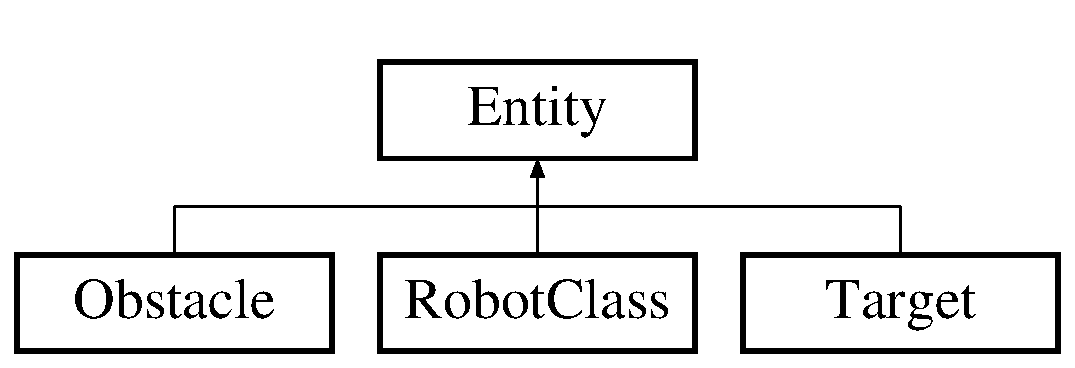
\includegraphics[height=2.000000cm]{classEntity}
\end{center}
\end{figure}
\subsection*{Public Member Functions}
\begin{DoxyCompactItemize}
\item 
\hyperlink{classEntity_a5c21cd9eab563bb481d9b5c65de91267}{Entity} (int pos\-X, int pos\-Y, int radius)
\item 
\hyperlink{classEntity_ad812a81e2ea7dfd1f4a0954c7ada44ad}{Entity} (\hyperlink{classVector2}{Vector2f}, int radius)
\item 
virtual void \hyperlink{classEntity_a00b6eeaf99b35c8f8b10b5fbfc1baf4f}{update} ()
\item 
virtual void \hyperlink{classEntity_af5ca41372ff108e4c044e8d927995a27}{render} ()
\item 
void \hyperlink{classEntity_a84fc43c322f66bf27ac6d90c328caf33}{translate} (\hyperlink{classVector2}{Vector2}$<$ int $>$ const \&shift)
\item 
void \hyperlink{classEntity_a1124a22e501d751041e41036af568ce6}{translate} (\hyperlink{classVector2}{Vector2f} const \&shift)
\item 
void \hyperlink{classEntity_a7d7233e4e9a8d9557648aab4612f0f3b}{translate} (int x, int y)
\item 
void \hyperlink{classEntity_a563fef5599c6da424fe656622b9d9324}{rotate} (float angle)
\item 
void \hyperlink{classEntity_ae9392a8133e210ad016f8e4ea4d63290}{rotate\-Rad} (float angle)
\item 
\hyperlink{classVector2}{Vector2f} \hyperlink{classEntity_ac45ad78fd8ef0d9938c1351798c181ab}{get\-Position} () const 
\item 
void \hyperlink{classEntity_a8c26c471c1f3e3a804d460533199bebf}{set\-Position} (\hyperlink{classVector2}{Vector2f} const \&)
\item 
\hyperlink{classVector2}{Vector2f} \hyperlink{classEntity_a899a2b90a1d7e26205095cad1d32a6d3}{get\-Orientation} () const 
\item 
void \hyperlink{classEntity_ac3c275ddf145d28416cdb6d0aad10ebf}{set\-Orientation} (\hyperlink{classVector2}{Vector2f} const \&)
\item 
float \hyperlink{classEntity_a35d819a8e850200d9734dace476d602a}{get\-Rotation} () const 
\item 
void \hyperlink{classEntity_a7d1e27098cf98b5e6fb6043263217315}{set\-Rotation} (float)
\item 
int \hyperlink{classEntity_ab9995764cb54c34e3715f7089a8e1714}{get\-Speed} () const 
\item 
void \hyperlink{classEntity_a2c6aaac44b0994328567b0311849c627}{set\-Speed} (int)
\item 
\hyperlink{classVector2}{Vector2f} \hyperlink{classEntity_a0217810f5096f6c0d04212d3cc1a935a}{get\-Velocity} () const 
\item 
void \hyperlink{classEntity_a03b1fc7ec44fe29fb946b86d6fe65842}{set\-Velocity} (\hyperlink{classVector2}{Vector2f} const \&)
\item 
bool \hyperlink{classEntity_a634c100994978b5ee96f8802e052a2d4}{collide} (\hyperlink{classEntity}{Entity} $\ast$other\-Entity)
\item 
bool \hyperlink{classEntity_a5591db8c22280b2157794be2841cb5a2}{bounds\-Check} ()
\item 
int \hyperlink{classEntity_ac2f290a20927f548e8742976b222a556}{get\-Radius} () const 
\item 
void \hyperlink{classEntity_ae5e084e71667daf1b18fc94b2cb8f363}{set\-Radius} (int)
\item 
unsigned int \hyperlink{classEntity_a69bd5fbeece40ba87d1e6f693f41d9ff}{get\-I\-D} ()
\item 
void \hyperlink{classEntity_a4992b9b8d1d9ef8f6d90ee20a053262c}{set\-Color} (\hyperlink{classColor}{Color} new\-Color)
\item 
\hyperlink{classColor}{Color} \hyperlink{classEntity_a9e60f2350275170500f33bcb8e57f3bc}{get\-Color} ()
\item 
void \hyperlink{classEntity_a4ff4124f2dfef873a2219b68f17bdfe5}{mark\-For\-Deletion} ()
\item 
virtual void \hyperlink{classEntity_a8e8ddac9be28d59f187a51e0fca0f056}{on\-Collide} (\hyperlink{classEntity}{Entity} $\ast$other\-Entity)
\item 
void \hyperlink{classEntity_a571c43e10649639994469f4229078fa0}{wall\-Collide} ()
\end{DoxyCompactItemize}
\subsection*{Protected Attributes}
\begin{DoxyCompactItemize}
\item 
\hypertarget{classEntity_a6af9d6498134ad0906011778bc5736db}{\hyperlink{classVector2}{Vector2f} {\bfseries position}}\label{classEntity_a6af9d6498134ad0906011778bc5736db}

\item 
\hypertarget{classEntity_acd7af12063926ab8cd654539328e5532}{int {\bfseries radius}}\label{classEntity_acd7af12063926ab8cd654539328e5532}

\item 
\hypertarget{classEntity_a5fa136f1d80e45ecf5c44199684af15d}{\hyperlink{classVector2}{Vector2f} {\bfseries orientation}}\label{classEntity_a5fa136f1d80e45ecf5c44199684af15d}

\item 
\hypertarget{classEntity_aa384ccfdaba36b1ff5f5db51ec3cdcb1}{float {\bfseries rotation}}\label{classEntity_aa384ccfdaba36b1ff5f5db51ec3cdcb1}

\item 
\hypertarget{classEntity_a12ea871d945d59cbf57b8f8f7d2179ed}{int {\bfseries speed}}\label{classEntity_a12ea871d945d59cbf57b8f8f7d2179ed}

\item 
\hypertarget{classEntity_a89d61354233997a696f1e0f82ecb9372}{\hyperlink{classVector2}{Vector2f} {\bfseries velocity}}\label{classEntity_a89d61354233997a696f1e0f82ecb9372}

\item 
\hypertarget{classEntity_aedfb34471b8e55194d5c93603ed23158}{unsigned int {\bfseries entity\-I\-D}}\label{classEntity_aedfb34471b8e55194d5c93603ed23158}

\item 
\hypertarget{classEntity_a2b8ccf8a215e4880a123b1c452438b01}{bool {\bfseries set\-For\-Deletion}}\label{classEntity_a2b8ccf8a215e4880a123b1c452438b01}

\item 
\hypertarget{classEntity_a98cdd3a9cc6efbecde0ad90ef349574c}{\hyperlink{classColor}{Color} {\bfseries rgb}}\label{classEntity_a98cdd3a9cc6efbecde0ad90ef349574c}

\end{DoxyCompactItemize}
\subsection*{Friends}
\begin{DoxyCompactItemize}
\item 
\hypertarget{classEntity_a6f579cda6059d102e9074e11a27e0282}{class {\bfseries Entity\-Manager}}\label{classEntity_a6f579cda6059d102e9074e11a27e0282}

\end{DoxyCompactItemize}


\subsection{Detailed Description}
This is the base class for all Entities. Robots, targets, and obstacles are all derived from this class. 

\begin{DoxyAuthor}{Author}
Dennis Ehrhardt 

Evan Stuempfig 

Andrew Hartfiel 

David Tran 
\end{DoxyAuthor}


\subsection{Constructor \& Destructor Documentation}
\hypertarget{classEntity_a5c21cd9eab563bb481d9b5c65de91267}{\index{Entity@{Entity}!Entity@{Entity}}
\index{Entity@{Entity}!Entity@{Entity}}
\subsubsection[{Entity}]{\setlength{\rightskip}{0pt plus 5cm}Entity\-::\-Entity (
\begin{DoxyParamCaption}
\item[{int}]{pos\-X, }
\item[{int}]{pos\-Y, }
\item[{int}]{radius}
\end{DoxyParamCaption}
)}}\label{classEntity_a5c21cd9eab563bb481d9b5c65de91267}
This constructor requires three parameters\-: x position, y position, and radius. 
\begin{DoxyParams}{Parameters}
{\em pos\-X} & the x position in pixels \\
\hline
{\em pos\-Y} & the y position in pixels \\
\hline
{\em radius} & the radius in pixels \\
\hline
\end{DoxyParams}
\hypertarget{classEntity_ad812a81e2ea7dfd1f4a0954c7ada44ad}{\index{Entity@{Entity}!Entity@{Entity}}
\index{Entity@{Entity}!Entity@{Entity}}
\subsubsection[{Entity}]{\setlength{\rightskip}{0pt plus 5cm}Entity\-::\-Entity (
\begin{DoxyParamCaption}
\item[{{\bf Vector2f}}]{vector\-In, }
\item[{int}]{radius}
\end{DoxyParamCaption}
)}}\label{classEntity_ad812a81e2ea7dfd1f4a0954c7ada44ad}
This constructor requires two parameters\-: location and radius. 
\begin{DoxyParams}{Parameters}
{\em location} & the x and y position in pixels as a \hyperlink{classVector2}{Vector2} \\
\hline
{\em radius} & the radius in pixels \\
\hline
\end{DoxyParams}


\subsection{Member Function Documentation}
\hypertarget{classEntity_a5591db8c22280b2157794be2841cb5a2}{\index{Entity@{Entity}!bounds\-Check@{bounds\-Check}}
\index{bounds\-Check@{bounds\-Check}!Entity@{Entity}}
\subsubsection[{bounds\-Check}]{\setlength{\rightskip}{0pt plus 5cm}bool Entity\-::bounds\-Check (
\begin{DoxyParamCaption}
{}
\end{DoxyParamCaption}
)}}\label{classEntity_a5591db8c22280b2157794be2841cb5a2}
Check that the entity is within the bounds of the map if it is not in bounds, it is brought in bounds \begin{DoxyReturn}{Returns}
False if out of bounds and brought back, True if originally in bounds 
\end{DoxyReturn}
\hypertarget{classEntity_a634c100994978b5ee96f8802e052a2d4}{\index{Entity@{Entity}!collide@{collide}}
\index{collide@{collide}!Entity@{Entity}}
\subsubsection[{collide}]{\setlength{\rightskip}{0pt plus 5cm}bool Entity\-::collide (
\begin{DoxyParamCaption}
\item[{{\bf Entity} $\ast$}]{other\-Entity}
\end{DoxyParamCaption}
)}}\label{classEntity_a634c100994978b5ee96f8802e052a2d4}
Check if there is a collision with another entity 
\begin{DoxyParams}{Parameters}
{\em other\-Entity} & the other entity \\
\hline
\end{DoxyParams}
\begin{DoxyReturn}{Returns}
True if collided, False otherwise 
\end{DoxyReturn}
\hypertarget{classEntity_a9e60f2350275170500f33bcb8e57f3bc}{\index{Entity@{Entity}!get\-Color@{get\-Color}}
\index{get\-Color@{get\-Color}!Entity@{Entity}}
\subsubsection[{get\-Color}]{\setlength{\rightskip}{0pt plus 5cm}{\bf Color} Entity\-::get\-Color (
\begin{DoxyParamCaption}
{}
\end{DoxyParamCaption}
)}}\label{classEntity_a9e60f2350275170500f33bcb8e57f3bc}
Get the color of the entity as R\-G\-B floats \begin{DoxyReturn}{Returns}
The color makeup of the entity 
\end{DoxyReturn}
\hypertarget{classEntity_a69bd5fbeece40ba87d1e6f693f41d9ff}{\index{Entity@{Entity}!get\-I\-D@{get\-I\-D}}
\index{get\-I\-D@{get\-I\-D}!Entity@{Entity}}
\subsubsection[{get\-I\-D}]{\setlength{\rightskip}{0pt plus 5cm}unsigned int Entity\-::get\-I\-D (
\begin{DoxyParamCaption}
{}
\end{DoxyParamCaption}
)}}\label{classEntity_a69bd5fbeece40ba87d1e6f693f41d9ff}
Get the I\-D of the entity \begin{DoxyReturn}{Returns}
The I\-D (int) 
\end{DoxyReturn}
\hypertarget{classEntity_a899a2b90a1d7e26205095cad1d32a6d3}{\index{Entity@{Entity}!get\-Orientation@{get\-Orientation}}
\index{get\-Orientation@{get\-Orientation}!Entity@{Entity}}
\subsubsection[{get\-Orientation}]{\setlength{\rightskip}{0pt plus 5cm}{\bf Vector2f} Entity\-::get\-Orientation (
\begin{DoxyParamCaption}
{}
\end{DoxyParamCaption}
) const}}\label{classEntity_a899a2b90a1d7e26205095cad1d32a6d3}
Get the orientation of the entity \begin{DoxyReturn}{Returns}
The orientation (\hyperlink{classVector2}{Vector2}) 
\end{DoxyReturn}
\hypertarget{classEntity_ac45ad78fd8ef0d9938c1351798c181ab}{\index{Entity@{Entity}!get\-Position@{get\-Position}}
\index{get\-Position@{get\-Position}!Entity@{Entity}}
\subsubsection[{get\-Position}]{\setlength{\rightskip}{0pt plus 5cm}{\bf Vector2f} Entity\-::get\-Position (
\begin{DoxyParamCaption}
{}
\end{DoxyParamCaption}
) const}}\label{classEntity_ac45ad78fd8ef0d9938c1351798c181ab}
Get the position of the center \begin{DoxyReturn}{Returns}
The position (\hyperlink{classVector2}{Vector2}) 
\end{DoxyReturn}
\hypertarget{classEntity_ac2f290a20927f548e8742976b222a556}{\index{Entity@{Entity}!get\-Radius@{get\-Radius}}
\index{get\-Radius@{get\-Radius}!Entity@{Entity}}
\subsubsection[{get\-Radius}]{\setlength{\rightskip}{0pt plus 5cm}int Entity\-::get\-Radius (
\begin{DoxyParamCaption}
{}
\end{DoxyParamCaption}
) const}}\label{classEntity_ac2f290a20927f548e8742976b222a556}
Get the radius of the entity in pixels \begin{DoxyReturn}{Returns}
The radius (int) 
\end{DoxyReturn}
\hypertarget{classEntity_a35d819a8e850200d9734dace476d602a}{\index{Entity@{Entity}!get\-Rotation@{get\-Rotation}}
\index{get\-Rotation@{get\-Rotation}!Entity@{Entity}}
\subsubsection[{get\-Rotation}]{\setlength{\rightskip}{0pt plus 5cm}float Entity\-::get\-Rotation (
\begin{DoxyParamCaption}
{}
\end{DoxyParamCaption}
) const}}\label{classEntity_a35d819a8e850200d9734dace476d602a}
Get the current speed in pixels per second \begin{DoxyReturn}{Returns}
The speed (int) 
\end{DoxyReturn}
\hypertarget{classEntity_ab9995764cb54c34e3715f7089a8e1714}{\index{Entity@{Entity}!get\-Speed@{get\-Speed}}
\index{get\-Speed@{get\-Speed}!Entity@{Entity}}
\subsubsection[{get\-Speed}]{\setlength{\rightskip}{0pt plus 5cm}int Entity\-::get\-Speed (
\begin{DoxyParamCaption}
{}
\end{DoxyParamCaption}
) const}}\label{classEntity_ab9995764cb54c34e3715f7089a8e1714}
Get the current speed in pixels per second \begin{DoxyReturn}{Returns}
The speed (int) 
\end{DoxyReturn}
\hypertarget{classEntity_a0217810f5096f6c0d04212d3cc1a935a}{\index{Entity@{Entity}!get\-Velocity@{get\-Velocity}}
\index{get\-Velocity@{get\-Velocity}!Entity@{Entity}}
\subsubsection[{get\-Velocity}]{\setlength{\rightskip}{0pt plus 5cm}{\bf Vector2f} Entity\-::get\-Velocity (
\begin{DoxyParamCaption}
{}
\end{DoxyParamCaption}
) const}}\label{classEntity_a0217810f5096f6c0d04212d3cc1a935a}
Get the velocity of the entity in pixels per second \begin{DoxyReturn}{Returns}
The velocity (\hyperlink{classVector2}{Vector2}) 
\end{DoxyReturn}
\hypertarget{classEntity_a4ff4124f2dfef873a2219b68f17bdfe5}{\index{Entity@{Entity}!mark\-For\-Deletion@{mark\-For\-Deletion}}
\index{mark\-For\-Deletion@{mark\-For\-Deletion}!Entity@{Entity}}
\subsubsection[{mark\-For\-Deletion}]{\setlength{\rightskip}{0pt plus 5cm}void Entity\-::mark\-For\-Deletion (
\begin{DoxyParamCaption}
{}
\end{DoxyParamCaption}
)}}\label{classEntity_a4ff4124f2dfef873a2219b68f17bdfe5}
Tell the \hyperlink{classEntityManager}{Entity\-Manager} to delete this object \hypertarget{classEntity_a8e8ddac9be28d59f187a51e0fca0f056}{\index{Entity@{Entity}!on\-Collide@{on\-Collide}}
\index{on\-Collide@{on\-Collide}!Entity@{Entity}}
\subsubsection[{on\-Collide}]{\setlength{\rightskip}{0pt plus 5cm}void Entity\-::on\-Collide (
\begin{DoxyParamCaption}
\item[{{\bf Entity} $\ast$}]{other\-Entity}
\end{DoxyParamCaption}
)\hspace{0.3cm}{\ttfamily [virtual]}}}\label{classEntity_a8e8ddac9be28d59f187a51e0fca0f056}
Called when this entity collides with another 
\begin{DoxyParams}{Parameters}
{\em other\-Entity} & the other entity \\
\hline
\end{DoxyParams}


Reimplemented in \hyperlink{classRobotClass_a84067f1a5a37b6a7113032e08daad9f2}{Robot\-Class}.

\hypertarget{classEntity_af5ca41372ff108e4c044e8d927995a27}{\index{Entity@{Entity}!render@{render}}
\index{render@{render}!Entity@{Entity}}
\subsubsection[{render}]{\setlength{\rightskip}{0pt plus 5cm}void Entity\-::render (
\begin{DoxyParamCaption}
{}
\end{DoxyParamCaption}
)\hspace{0.3cm}{\ttfamily [virtual]}}}\label{classEntity_af5ca41372ff108e4c044e8d927995a27}
Draw the entity on the screen 

Reimplemented in \hyperlink{classRobotClass_a739de3580edf634c29e1185364d96d32}{Robot\-Class}, \hyperlink{classObstacle_ab5dc508912a5c772e8a9c732c9db5c24}{Obstacle}, and \hyperlink{classTarget_a5230b99d26495595cf6879dd6816277a}{Target}.

\hypertarget{classEntity_a563fef5599c6da424fe656622b9d9324}{\index{Entity@{Entity}!rotate@{rotate}}
\index{rotate@{rotate}!Entity@{Entity}}
\subsubsection[{rotate}]{\setlength{\rightskip}{0pt plus 5cm}void Entity\-::rotate (
\begin{DoxyParamCaption}
\item[{float}]{angle}
\end{DoxyParamCaption}
)}}\label{classEntity_a563fef5599c6da424fe656622b9d9324}
Rotate the entity's orientation in degrees 
\begin{DoxyParams}{Parameters}
{\em angle} & how much to rotate the entity in degrees \\
\hline
\end{DoxyParams}
\hypertarget{classEntity_ae9392a8133e210ad016f8e4ea4d63290}{\index{Entity@{Entity}!rotate\-Rad@{rotate\-Rad}}
\index{rotate\-Rad@{rotate\-Rad}!Entity@{Entity}}
\subsubsection[{rotate\-Rad}]{\setlength{\rightskip}{0pt plus 5cm}void Entity\-::rotate\-Rad (
\begin{DoxyParamCaption}
\item[{float}]{angle}
\end{DoxyParamCaption}
)}}\label{classEntity_ae9392a8133e210ad016f8e4ea4d63290}
Rotate the entity's orientation 
\begin{DoxyParams}{Parameters}
{\em angle} & how much to rotate the entity in radians \\
\hline
\end{DoxyParams}
\hypertarget{classEntity_a4992b9b8d1d9ef8f6d90ee20a053262c}{\index{Entity@{Entity}!set\-Color@{set\-Color}}
\index{set\-Color@{set\-Color}!Entity@{Entity}}
\subsubsection[{set\-Color}]{\setlength{\rightskip}{0pt plus 5cm}void Entity\-::set\-Color (
\begin{DoxyParamCaption}
\item[{{\bf Color}}]{new\-Color}
\end{DoxyParamCaption}
)}}\label{classEntity_a4992b9b8d1d9ef8f6d90ee20a053262c}
Change the color of the entity 
\begin{DoxyParams}{Parameters}
{\em new\-Color} & the new color of the entity \\
\hline
\end{DoxyParams}
\hypertarget{classEntity_ac3c275ddf145d28416cdb6d0aad10ebf}{\index{Entity@{Entity}!set\-Orientation@{set\-Orientation}}
\index{set\-Orientation@{set\-Orientation}!Entity@{Entity}}
\subsubsection[{set\-Orientation}]{\setlength{\rightskip}{0pt plus 5cm}void Entity\-::set\-Orientation (
\begin{DoxyParamCaption}
\item[{{\bf Vector2f} const \&}]{new\-Orientation}
\end{DoxyParamCaption}
)}}\label{classEntity_ac3c275ddf145d28416cdb6d0aad10ebf}
Set the orientation of entity 
\begin{DoxyParams}{Parameters}
{\em new\-Orientation} & the new orientation of the entity \\
\hline
\end{DoxyParams}
\hypertarget{classEntity_a8c26c471c1f3e3a804d460533199bebf}{\index{Entity@{Entity}!set\-Position@{set\-Position}}
\index{set\-Position@{set\-Position}!Entity@{Entity}}
\subsubsection[{set\-Position}]{\setlength{\rightskip}{0pt plus 5cm}void Entity\-::set\-Position (
\begin{DoxyParamCaption}
\item[{{\bf Vector2f} const \&}]{new\-Position}
\end{DoxyParamCaption}
)}}\label{classEntity_a8c26c471c1f3e3a804d460533199bebf}
Set the position of the center 
\begin{DoxyParams}{Parameters}
{\em new\-Position} & the new position of the center \\
\hline
\end{DoxyParams}
\hypertarget{classEntity_ae5e084e71667daf1b18fc94b2cb8f363}{\index{Entity@{Entity}!set\-Radius@{set\-Radius}}
\index{set\-Radius@{set\-Radius}!Entity@{Entity}}
\subsubsection[{set\-Radius}]{\setlength{\rightskip}{0pt plus 5cm}void Entity\-::set\-Radius (
\begin{DoxyParamCaption}
\item[{int}]{new\-Radius}
\end{DoxyParamCaption}
)}}\label{classEntity_ae5e084e71667daf1b18fc94b2cb8f363}
Set the radius of the entity in pixels 
\begin{DoxyParams}{Parameters}
{\em new\-Radius} & the new radius of the entity \\
\hline
\end{DoxyParams}
\hypertarget{classEntity_a7d1e27098cf98b5e6fb6043263217315}{\index{Entity@{Entity}!set\-Rotation@{set\-Rotation}}
\index{set\-Rotation@{set\-Rotation}!Entity@{Entity}}
\subsubsection[{set\-Rotation}]{\setlength{\rightskip}{0pt plus 5cm}void Entity\-::set\-Rotation (
\begin{DoxyParamCaption}
\item[{float}]{new\-Rotation}
\end{DoxyParamCaption}
)}}\label{classEntity_a7d1e27098cf98b5e6fb6043263217315}
Set the rotation of entity 
\begin{DoxyParams}{Parameters}
{\em new\-Rotation} & the new rotation of the entity \\
\hline
\end{DoxyParams}
\hypertarget{classEntity_a2c6aaac44b0994328567b0311849c627}{\index{Entity@{Entity}!set\-Speed@{set\-Speed}}
\index{set\-Speed@{set\-Speed}!Entity@{Entity}}
\subsubsection[{set\-Speed}]{\setlength{\rightskip}{0pt plus 5cm}void Entity\-::set\-Speed (
\begin{DoxyParamCaption}
\item[{int}]{new\-Speed}
\end{DoxyParamCaption}
)}}\label{classEntity_a2c6aaac44b0994328567b0311849c627}
Set the current speed in pixels per second 
\begin{DoxyParams}{Parameters}
{\em new\-Speed} & the new speed of the entity \\
\hline
\end{DoxyParams}
\begin{DoxyNote}{Note}
values below 0 are rounded to 0 
\end{DoxyNote}
\hypertarget{classEntity_a03b1fc7ec44fe29fb946b86d6fe65842}{\index{Entity@{Entity}!set\-Velocity@{set\-Velocity}}
\index{set\-Velocity@{set\-Velocity}!Entity@{Entity}}
\subsubsection[{set\-Velocity}]{\setlength{\rightskip}{0pt plus 5cm}void Entity\-::set\-Velocity (
\begin{DoxyParamCaption}
\item[{{\bf Vector2f} const \&}]{new\-Velocity}
\end{DoxyParamCaption}
)}}\label{classEntity_a03b1fc7ec44fe29fb946b86d6fe65842}
Set the velocity of the entity in pixels per second 
\begin{DoxyParams}{Parameters}
{\em new\-Velocity} & the new velocity of the entity \\
\hline
\end{DoxyParams}
\hypertarget{classEntity_a84fc43c322f66bf27ac6d90c328caf33}{\index{Entity@{Entity}!translate@{translate}}
\index{translate@{translate}!Entity@{Entity}}
\subsubsection[{translate}]{\setlength{\rightskip}{0pt plus 5cm}void Entity\-::translate (
\begin{DoxyParamCaption}
\item[{{\bf Vector2}$<$ int $>$ const \&}]{shift}
\end{DoxyParamCaption}
)}}\label{classEntity_a84fc43c322f66bf27ac6d90c328caf33}
Shift the entity to a new position 
\begin{DoxyParams}{Parameters}
{\em shift} & how much to shift the entity by in pixels as a \hyperlink{classVector2}{Vector2} \\
\hline
\end{DoxyParams}
\hypertarget{classEntity_a1124a22e501d751041e41036af568ce6}{\index{Entity@{Entity}!translate@{translate}}
\index{translate@{translate}!Entity@{Entity}}
\subsubsection[{translate}]{\setlength{\rightskip}{0pt plus 5cm}void Entity\-::translate (
\begin{DoxyParamCaption}
\item[{{\bf Vector2f} const \&}]{shift}
\end{DoxyParamCaption}
)}}\label{classEntity_a1124a22e501d751041e41036af568ce6}
Shift the entity to a new position 
\begin{DoxyParams}{Parameters}
{\em shift} & how much to shift the entity by in pixels as a \hyperlink{classVector2}{Vector2} \\
\hline
\end{DoxyParams}
\hypertarget{classEntity_a7d7233e4e9a8d9557648aab4612f0f3b}{\index{Entity@{Entity}!translate@{translate}}
\index{translate@{translate}!Entity@{Entity}}
\subsubsection[{translate}]{\setlength{\rightskip}{0pt plus 5cm}void Entity\-::translate (
\begin{DoxyParamCaption}
\item[{int}]{x, }
\item[{int}]{y}
\end{DoxyParamCaption}
)}}\label{classEntity_a7d7233e4e9a8d9557648aab4612f0f3b}
Shift the entity to a new position 
\begin{DoxyParams}{Parameters}
{\em x\-Shift} & how much to shift the entity in the x direction in pixels \\
\hline
{\em y\-Shift} & how much to shift the entity in the y direction in pixels \\
\hline
\end{DoxyParams}
\hypertarget{classEntity_a00b6eeaf99b35c8f8b10b5fbfc1baf4f}{\index{Entity@{Entity}!update@{update}}
\index{update@{update}!Entity@{Entity}}
\subsubsection[{update}]{\setlength{\rightskip}{0pt plus 5cm}void Entity\-::update (
\begin{DoxyParamCaption}
{}
\end{DoxyParamCaption}
)\hspace{0.3cm}{\ttfamily [virtual]}}}\label{classEntity_a00b6eeaf99b35c8f8b10b5fbfc1baf4f}
Update the entity's position and behavior 

Reimplemented in \hyperlink{classRobotClass_a1d4d22f50854bf62af206d71f25c2a52}{Robot\-Class}, \hyperlink{classObstacle_a3fe041a93f5b2e9e5c5750bcef2382a4}{Obstacle}, and \hyperlink{classTarget_a33e3e447eeba8ded77cb3becf30f98d3}{Target}.

\hypertarget{classEntity_a571c43e10649639994469f4229078fa0}{\index{Entity@{Entity}!wall\-Collide@{wall\-Collide}}
\index{wall\-Collide@{wall\-Collide}!Entity@{Entity}}
\subsubsection[{wall\-Collide}]{\setlength{\rightskip}{0pt plus 5cm}void Entity\-::wall\-Collide (
\begin{DoxyParamCaption}
{}
\end{DoxyParamCaption}
)}}\label{classEntity_a571c43e10649639994469f4229078fa0}
Called at every update to determine which wall(s) the entity is colliding with and adjust its orientation appropriately 

The documentation for this class was generated from the following files\-:\begin{DoxyCompactItemize}
\item 
Entity/Entity.\-h\item 
Entity/Entity.\-cpp\end{DoxyCompactItemize}

\hypertarget{classEntityManager}{\section{Entity\-Manager Class Reference}
\label{classEntityManager}\index{Entity\-Manager@{Entity\-Manager}}
}


This class is used to manage entities.  




{\ttfamily \#include $<$Entity\-Manager.\-h$>$}

\subsection*{Public Member Functions}
\begin{DoxyCompactItemize}
\item 
void \hyperlink{classEntityManager_abc6a2cc5077501f4b06d88f4ed3e7e31}{update} ()
\item 
void \hyperlink{classEntityManager_a663907dd48bbaf39344352a14b68d35a}{render} ()
\item 
void \hyperlink{classEntityManager_acc4cf521b2b9b33b37fd5685c2d1a504}{add} (\hyperlink{classEntity}{Entity} $\ast$)
\item 
void \hyperlink{classEntityManager_a322d6323d3d2b22581ca50efd1e253f5}{clear} ()
\item 
\hyperlink{classVector2}{Vector2f} \hyperlink{classEntityManager_a04a01dccea941da24815a4f58dd92a97}{homing\-Feedback} (int src, int dst)
\item 
unsigned int \hyperlink{classEntityManager_a2a13894e743374b43461f8586ab4880d}{get\-Entity\-I\-D} (\hyperlink{classEntity}{Entity} $\ast$entity)
\item 
\hyperlink{classEntity}{Entity} $\ast$ \hyperlink{classEntityManager_a2de0aa13460347a87b568a37cb0b11fc}{get\-Entity} (unsigned int id)
\item 
bool \hyperlink{classEntityManager_a68bec5ed352a62adc662166c0a09e5e8}{collide\-With\-Anything} (\hyperlink{classEntity}{Entity} $\ast$)
\item 
\hypertarget{classEntityManager_ad54b4992602323278fef716e20064554}{void {\bfseries collide} ()}\label{classEntityManager_ad54b4992602323278fef716e20064554}

\end{DoxyCompactItemize}
\subsection*{Static Public Member Functions}
\begin{DoxyCompactItemize}
\item 
\hypertarget{classEntityManager_a6d87bc4ad44459500e6a754de4724d1d}{static \hyperlink{classEntityManager}{Entity\-Manager} \& {\bfseries get\-Instance} ()}\label{classEntityManager_a6d87bc4ad44459500e6a754de4724d1d}

\end{DoxyCompactItemize}


\subsection{Detailed Description}
This class is used to manage entities. 

\begin{DoxyNote}{Note}
\hyperlink{classEntityManager}{Entity\-Manager} is a singleton class. 
\end{DoxyNote}
\begin{DoxyAuthor}{Author}
Dennis Ehrhardt 
\end{DoxyAuthor}


\subsection{Member Function Documentation}
\hypertarget{classEntityManager_acc4cf521b2b9b33b37fd5685c2d1a504}{\index{Entity\-Manager@{Entity\-Manager}!add@{add}}
\index{add@{add}!EntityManager@{Entity\-Manager}}
\subsubsection[{add}]{\setlength{\rightskip}{0pt plus 5cm}void Entity\-Manager\-::add (
\begin{DoxyParamCaption}
\item[{{\bf Entity} $\ast$}]{entity}
\end{DoxyParamCaption}
)}}\label{classEntityManager_acc4cf521b2b9b33b37fd5685c2d1a504}
Add a new entity to the manager 
\begin{DoxyParams}{Parameters}
{\em new\-Entity} & the new entity to add \\
\hline
\end{DoxyParams}
\hypertarget{classEntityManager_a322d6323d3d2b22581ca50efd1e253f5}{\index{Entity\-Manager@{Entity\-Manager}!clear@{clear}}
\index{clear@{clear}!EntityManager@{Entity\-Manager}}
\subsubsection[{clear}]{\setlength{\rightskip}{0pt plus 5cm}void Entity\-Manager\-::clear (
\begin{DoxyParamCaption}
{}
\end{DoxyParamCaption}
)}}\label{classEntityManager_a322d6323d3d2b22581ca50efd1e253f5}
Clear and delete all Entities in the Manager \hypertarget{classEntityManager_a68bec5ed352a62adc662166c0a09e5e8}{\index{Entity\-Manager@{Entity\-Manager}!collide\-With\-Anything@{collide\-With\-Anything}}
\index{collide\-With\-Anything@{collide\-With\-Anything}!EntityManager@{Entity\-Manager}}
\subsubsection[{collide\-With\-Anything}]{\setlength{\rightskip}{0pt plus 5cm}bool Entity\-Manager\-::collide\-With\-Anything (
\begin{DoxyParamCaption}
\item[{{\bf Entity} $\ast$}]{entity}
\end{DoxyParamCaption}
)}}\label{classEntityManager_a68bec5ed352a62adc662166c0a09e5e8}
Checks to see if the entity collides with anything 
\begin{DoxyParams}{Parameters}
{\em takes} & in an \hyperlink{classEntity}{Entity} to check if it collides with anything \\
\hline
\end{DoxyParams}
\begin{DoxyReturn}{Returns}
Returns true if it collides with another entity and false if it doesn't 
\end{DoxyReturn}
\hypertarget{classEntityManager_a2de0aa13460347a87b568a37cb0b11fc}{\index{Entity\-Manager@{Entity\-Manager}!get\-Entity@{get\-Entity}}
\index{get\-Entity@{get\-Entity}!EntityManager@{Entity\-Manager}}
\subsubsection[{get\-Entity}]{\setlength{\rightskip}{0pt plus 5cm}{\bf Entity} $\ast$ Entity\-Manager\-::get\-Entity (
\begin{DoxyParamCaption}
\item[{unsigned int}]{id}
\end{DoxyParamCaption}
)}}\label{classEntityManager_a2de0aa13460347a87b568a37cb0b11fc}
Gets the entity given an I\-D 
\begin{DoxyParams}{Parameters}
{\em id} & the id \\
\hline
\end{DoxyParams}
\begin{DoxyReturn}{Returns}
The entity, if it exists, N\-U\-L\-L if not (Entity$\ast$) 
\end{DoxyReturn}
\hypertarget{classEntityManager_a2a13894e743374b43461f8586ab4880d}{\index{Entity\-Manager@{Entity\-Manager}!get\-Entity\-I\-D@{get\-Entity\-I\-D}}
\index{get\-Entity\-I\-D@{get\-Entity\-I\-D}!EntityManager@{Entity\-Manager}}
\subsubsection[{get\-Entity\-I\-D}]{\setlength{\rightskip}{0pt plus 5cm}unsigned int Entity\-Manager\-::get\-Entity\-I\-D (
\begin{DoxyParamCaption}
\item[{{\bf Entity} $\ast$}]{entity}
\end{DoxyParamCaption}
)}}\label{classEntityManager_a2a13894e743374b43461f8586ab4880d}
Gets the I\-D of an entity 
\begin{DoxyParams}{Parameters}
{\em entity} & the entity \\
\hline
\end{DoxyParams}
\begin{DoxyReturn}{Returns}
The I\-D of the entity, if it exists, -\/1 if not (unsigned int) 
\end{DoxyReturn}
\hypertarget{classEntityManager_a04a01dccea941da24815a4f58dd92a97}{\index{Entity\-Manager@{Entity\-Manager}!homing\-Feedback@{homing\-Feedback}}
\index{homing\-Feedback@{homing\-Feedback}!EntityManager@{Entity\-Manager}}
\subsubsection[{homing\-Feedback}]{\setlength{\rightskip}{0pt plus 5cm}{\bf Vector2f} Entity\-Manager\-::homing\-Feedback (
\begin{DoxyParamCaption}
\item[{int}]{src, }
\item[{int}]{dst}
\end{DoxyParamCaption}
)}}\label{classEntityManager_a04a01dccea941da24815a4f58dd92a97}
Get the direction and distance from one entity to another 
\begin{DoxyParams}{Parameters}
{\em src} & the I\-D of the source object \\
\hline
{\em dst} & the I\-D of the destination object \\
\hline
\end{DoxyParams}
\begin{DoxyReturn}{Returns}
A the distance and direction (\hyperlink{classVector2}{Vector2}) 
\end{DoxyReturn}
\hypertarget{classEntityManager_a663907dd48bbaf39344352a14b68d35a}{\index{Entity\-Manager@{Entity\-Manager}!render@{render}}
\index{render@{render}!EntityManager@{Entity\-Manager}}
\subsubsection[{render}]{\setlength{\rightskip}{0pt plus 5cm}void Entity\-Manager\-::render (
\begin{DoxyParamCaption}
{}
\end{DoxyParamCaption}
)}}\label{classEntityManager_a663907dd48bbaf39344352a14b68d35a}
Draw all of the entities \hypertarget{classEntityManager_abc6a2cc5077501f4b06d88f4ed3e7e31}{\index{Entity\-Manager@{Entity\-Manager}!update@{update}}
\index{update@{update}!EntityManager@{Entity\-Manager}}
\subsubsection[{update}]{\setlength{\rightskip}{0pt plus 5cm}void Entity\-Manager\-::update (
\begin{DoxyParamCaption}
{}
\end{DoxyParamCaption}
)}}\label{classEntityManager_abc6a2cc5077501f4b06d88f4ed3e7e31}
Call the update method of all entities and run collisions 

The documentation for this class was generated from the following files\-:\begin{DoxyCompactItemize}
\item 
Entity/Entity\-Manager.\-h\item 
Entity/Entity\-Manager.\-cpp\end{DoxyCompactItemize}

\hypertarget{classEntityTests}{\section{Entity\-Tests Class Reference}
\label{classEntityTests}\index{Entity\-Tests@{Entity\-Tests}}
}
Inheritance diagram for Entity\-Tests\-:\begin{figure}[H]
\begin{center}
\leavevmode
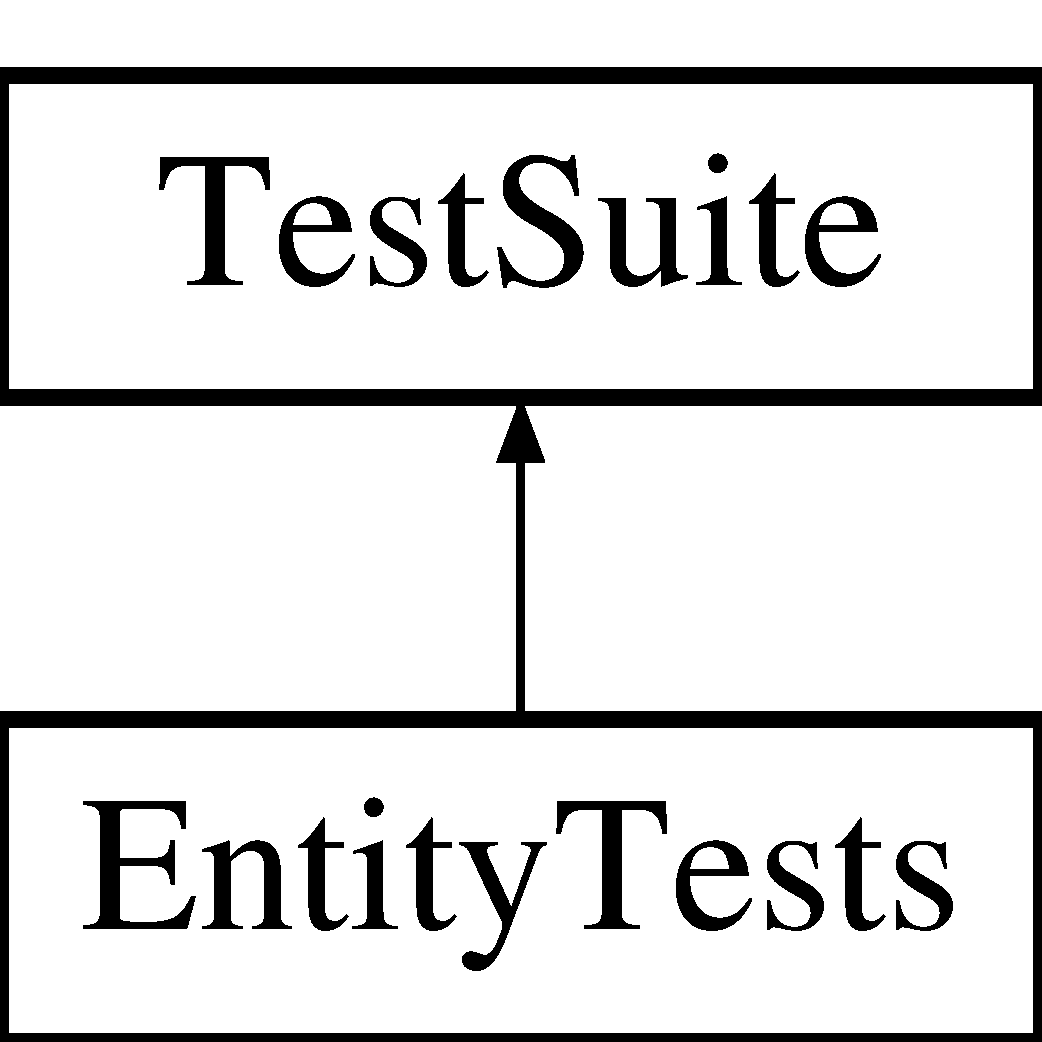
\includegraphics[height=2.000000cm]{classEntityTests}
\end{center}
\end{figure}
\subsection*{Public Member Functions}
\begin{DoxyCompactItemize}
\item 
\hypertarget{classEntityTests_a4b80612f9df50c754b3ac3171e78755a}{void {\bfseries Test\-\_\-\-Get\-\_\-\-Set\-\_\-\-Orientation} ()}\label{classEntityTests_a4b80612f9df50c754b3ac3171e78755a}

\item 
\hypertarget{classEntityTests_aef1302b74489aa166bcdef3bad7b4715}{void {\bfseries Test\-\_\-\-Rotate\-\_\-\-Rad} ()}\label{classEntityTests_aef1302b74489aa166bcdef3bad7b4715}

\item 
\hypertarget{classEntityTests_a7ec5053f823a1161afe6cc7a60fdd86b}{void {\bfseries Test\-\_\-\-Rotate} ()}\label{classEntityTests_a7ec5053f823a1161afe6cc7a60fdd86b}

\item 
\hypertarget{classEntityTests_ad56e4efd080a454d757def1d9e7a4e1d}{void {\bfseries Test\-\_\-\-Translate\-\_\-\-Int\-\_\-\-Vec} ()}\label{classEntityTests_ad56e4efd080a454d757def1d9e7a4e1d}

\item 
\hypertarget{classEntityTests_a45140149055d3f6a9242ce0a30f20f73}{void {\bfseries Test\-\_\-\-Translate\-\_\-\-Float\-\_\-\-Vec} ()}\label{classEntityTests_a45140149055d3f6a9242ce0a30f20f73}

\item 
\hypertarget{classEntityTests_abd0c1ad16d97fe93f38136aff2b5f76e}{void {\bfseries Test\-\_\-\-Translate\-\_\-\-Comp} ()}\label{classEntityTests_abd0c1ad16d97fe93f38136aff2b5f76e}

\item 
\hypertarget{classEntityTests_a3d375bebf514f85133a01943356be591}{void {\bfseries Test\-\_\-\-Get\-\_\-\-Set\-\_\-\-Radius} ()}\label{classEntityTests_a3d375bebf514f85133a01943356be591}

\item 
\hypertarget{classEntityTests_a1d042a2454be85bb48cfc99a2302723d}{void {\bfseries Test\-\_\-\-Get\-\_\-\-Set\-\_\-\-Speed} ()}\label{classEntityTests_a1d042a2454be85bb48cfc99a2302723d}

\item 
\hypertarget{classEntityTests_a543d15f2b57a3e1d70de4e5f30d055d5}{void {\bfseries Test\-\_\-\-Get\-\_\-\-Set\-\_\-\-Velocity} ()}\label{classEntityTests_a543d15f2b57a3e1d70de4e5f30d055d5}

\item 
\hypertarget{classEntityTests_aa071eb69b86308de0e948cc2ce8b63b2}{void {\bfseries Test\-\_\-\-Bounds\-Check} ()}\label{classEntityTests_aa071eb69b86308de0e948cc2ce8b63b2}

\item 
\hypertarget{classEntityTests_a2ee30a69ba16c465fe0b249500ba1b6d}{void {\bfseries Test\-\_\-\-Touch\-\_\-\-Sensor} ()}\label{classEntityTests_a2ee30a69ba16c465fe0b249500ba1b6d}

\item 
\hypertarget{classEntityTests_a39807fd0505ee320fdb2683ba67afd22}{void {\bfseries Test\-\_\-\-Collide} ()}\label{classEntityTests_a39807fd0505ee320fdb2683ba67afd22}

\item 
\hypertarget{classEntityTests_aceee224e305889de02c015c61888ee03}{void {\bfseries Test\-\_\-\-Get\-\_\-\-Set\-\_\-\-Position} ()}\label{classEntityTests_aceee224e305889de02c015c61888ee03}

\item 
\hypertarget{classEntityTests_adbbbe9abf38b242b9b0fb6979d988e88}{void {\bfseries Test\-\_\-\-Point\-\_\-\-At\-\_\-\-Target} ()}\label{classEntityTests_adbbbe9abf38b242b9b0fb6979d988e88}

\item 
\hypertarget{classEntityTests_a5330e1fa9789721c29c85bdb01e3d467}{void {\bfseries Test\-\_\-\-Home\-\_\-\-On\-\_\-\-Target} ()}\label{classEntityTests_a5330e1fa9789721c29c85bdb01e3d467}

\item 
\hypertarget{classEntityTests_ac7a90330b5be556829c9b15f614c7b5a}{void {\bfseries Test\-\_\-\-Robot\-\_\-\-Target\-\_\-\-Collide} ()}\label{classEntityTests_ac7a90330b5be556829c9b15f614c7b5a}

\end{DoxyCompactItemize}


The documentation for this class was generated from the following file\-:\begin{DoxyCompactItemize}
\item 
Entity\-Tests.\-h\end{DoxyCompactItemize}

\hypertarget{classObstacle}{\section{Obstacle Class Reference}
\label{classObstacle}\index{Obstacle@{Obstacle}}
}


The class for creating obstacles.  




{\ttfamily \#include $<$Obstacle.\-h$>$}

Inheritance diagram for Obstacle\-:\begin{figure}[H]
\begin{center}
\leavevmode
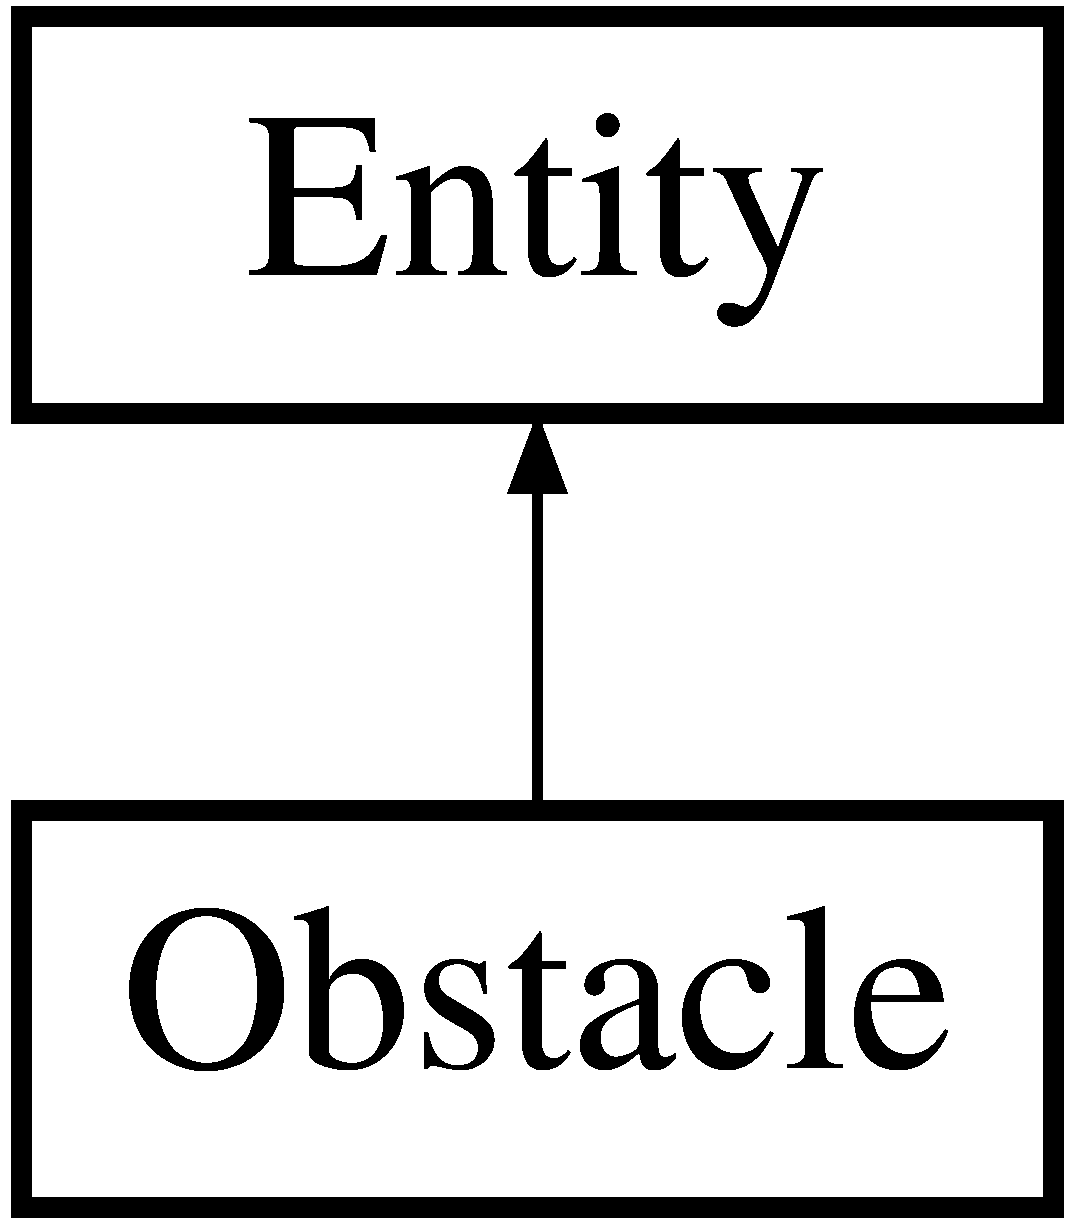
\includegraphics[height=2.000000cm]{classObstacle}
\end{center}
\end{figure}
\subsection*{Public Member Functions}
\begin{DoxyCompactItemize}
\item 
\hyperlink{classObstacle_a54f7a6e679d123958539eabe85694656}{Obstacle} (int pos\-X, int pos\-Y, int radius)
\item 
\hyperlink{classObstacle_a2ccff96a4ddb5aee99504a9f90061f32}{Obstacle} (\hyperlink{classVector2}{Vector2f} position, int radius)
\item 
void \hyperlink{classObstacle_a3fe041a93f5b2e9e5c5750bcef2382a4}{update} ()
\item 
void \hyperlink{classObstacle_ab5dc508912a5c772e8a9c732c9db5c24}{render} ()
\end{DoxyCompactItemize}
\subsection*{Additional Inherited Members}


\subsection{Detailed Description}
The class for creating obstacles. 

\begin{DoxyAuthor}{Author}
Dennis Ehrhardt 

Evan Stuempfig 

Andrew Hartfiel 

David Tran 
\end{DoxyAuthor}


\subsection{Constructor \& Destructor Documentation}
\hypertarget{classObstacle_a54f7a6e679d123958539eabe85694656}{\index{Obstacle@{Obstacle}!Obstacle@{Obstacle}}
\index{Obstacle@{Obstacle}!Obstacle@{Obstacle}}
\subsubsection[{Obstacle}]{\setlength{\rightskip}{0pt plus 5cm}Obstacle\-::\-Obstacle (
\begin{DoxyParamCaption}
\item[{int}]{pos\-X, }
\item[{int}]{pos\-Y, }
\item[{int}]{radius}
\end{DoxyParamCaption}
)\hspace{0.3cm}{\ttfamily [inline]}}}\label{classObstacle_a54f7a6e679d123958539eabe85694656}
This constructor requires three parameters\-: x position, y position, and radius. 
\begin{DoxyParams}{Parameters}
{\em pos\-X} & the x position in pixels \\
\hline
{\em pos\-Y} & the y position in pixels \\
\hline
{\em radius} & the radius in pixels \\
\hline
\end{DoxyParams}
\hypertarget{classObstacle_a2ccff96a4ddb5aee99504a9f90061f32}{\index{Obstacle@{Obstacle}!Obstacle@{Obstacle}}
\index{Obstacle@{Obstacle}!Obstacle@{Obstacle}}
\subsubsection[{Obstacle}]{\setlength{\rightskip}{0pt plus 5cm}Obstacle\-::\-Obstacle (
\begin{DoxyParamCaption}
\item[{{\bf Vector2f}}]{position, }
\item[{int}]{radius}
\end{DoxyParamCaption}
)\hspace{0.3cm}{\ttfamily [inline]}}}\label{classObstacle_a2ccff96a4ddb5aee99504a9f90061f32}
This constructor requires two parameters\-: location and radius. 
\begin{DoxyParams}{Parameters}
{\em location} & the x and y position in pixels as a \hyperlink{classVector2}{Vector2} \\
\hline
{\em radius} & the radius in pixels \\
\hline
\end{DoxyParams}


\subsection{Member Function Documentation}
\hypertarget{classObstacle_ab5dc508912a5c772e8a9c732c9db5c24}{\index{Obstacle@{Obstacle}!render@{render}}
\index{render@{render}!Obstacle@{Obstacle}}
\subsubsection[{render}]{\setlength{\rightskip}{0pt plus 5cm}void Obstacle\-::render (
\begin{DoxyParamCaption}
{}
\end{DoxyParamCaption}
)\hspace{0.3cm}{\ttfamily [virtual]}}}\label{classObstacle_ab5dc508912a5c772e8a9c732c9db5c24}
Draw the obstacle on the screen 

Reimplemented from \hyperlink{classEntity_af5ca41372ff108e4c044e8d927995a27}{Entity}.

\hypertarget{classObstacle_a3fe041a93f5b2e9e5c5750bcef2382a4}{\index{Obstacle@{Obstacle}!update@{update}}
\index{update@{update}!Obstacle@{Obstacle}}
\subsubsection[{update}]{\setlength{\rightskip}{0pt plus 5cm}void Obstacle\-::update (
\begin{DoxyParamCaption}
{}
\end{DoxyParamCaption}
)\hspace{0.3cm}{\ttfamily [virtual]}}}\label{classObstacle_a3fe041a93f5b2e9e5c5750bcef2382a4}
Update the obstacle's position and behavior 

Reimplemented from \hyperlink{classEntity_a00b6eeaf99b35c8f8b10b5fbfc1baf4f}{Entity}.



The documentation for this class was generated from the following files\-:\begin{DoxyCompactItemize}
\item 
Entity/Obstacle.\-h\item 
Entity/Obstacle.\-cpp\end{DoxyCompactItemize}

\hypertarget{classRobotClass}{\section{Robot\-Class Class Reference}
\label{classRobotClass}\index{Robot\-Class@{Robot\-Class}}
}


The class for creating robots.  




{\ttfamily \#include $<$Robot\-Class.\-h$>$}

Inheritance diagram for Robot\-Class\-:\begin{figure}[H]
\begin{center}
\leavevmode
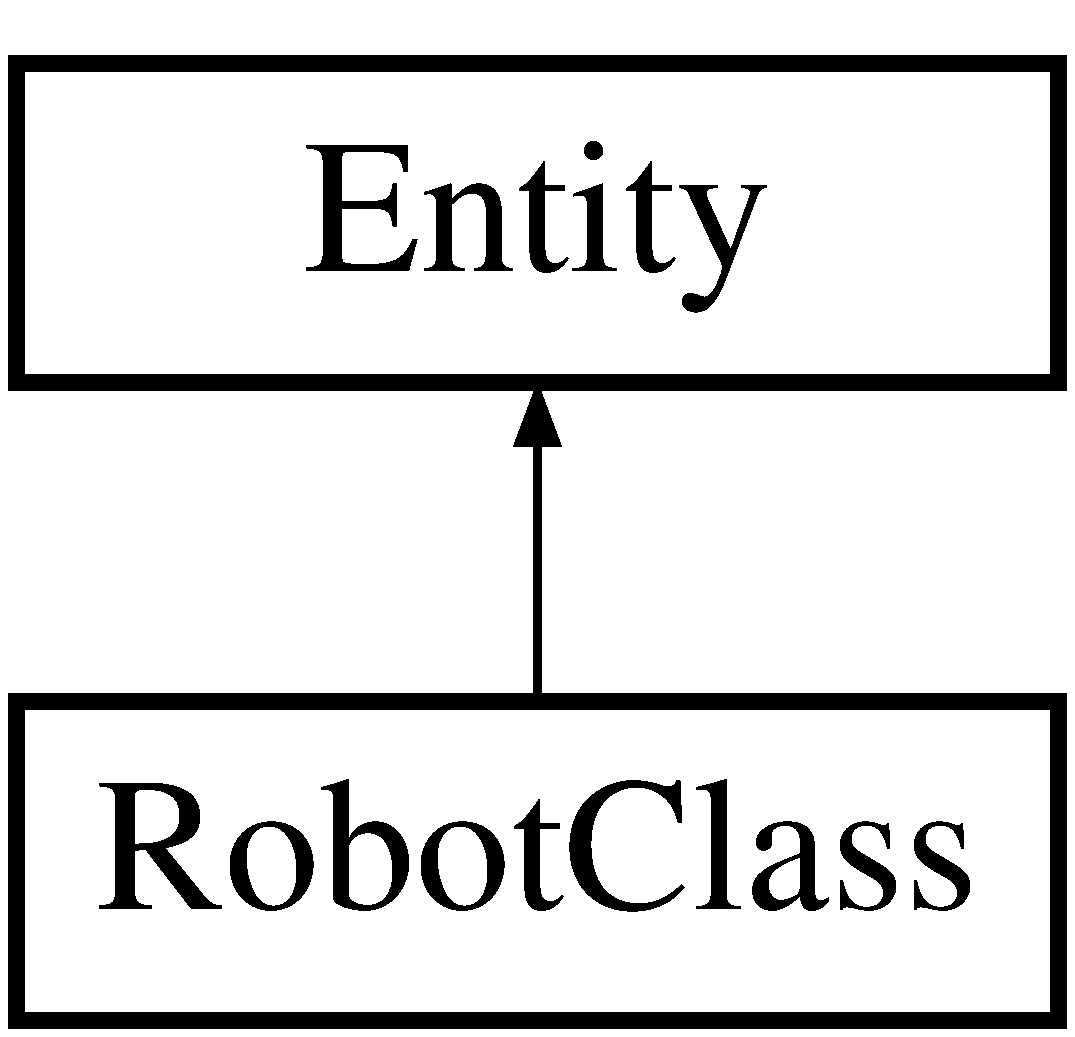
\includegraphics[height=2.000000cm]{classRobotClass}
\end{center}
\end{figure}
\subsection*{Public Member Functions}
\begin{DoxyCompactItemize}
\item 
\hyperlink{classRobotClass_a66fe919002ecfe53bb9ad55d7caf2279}{Robot\-Class} (int pos\-X, int pos\-Y, int radius)
\item 
\hyperlink{classRobotClass_a339a2ae3a897461d74684a3d6eea7f44}{Robot\-Class} (\hyperlink{classVector2}{Vector2f} position, int radius)
\item 
void \hyperlink{classRobotClass_a1d4d22f50854bf62af206d71f25c2a52}{update} ()
\item 
void \hyperlink{classRobotClass_a739de3580edf634c29e1185364d96d32}{render} ()
\item 
void \hyperlink{classRobotClass_ab1fe4c11b2a955eaa637024e2491175d}{point\-At\-Target} ()
\item 
\hyperlink{classVector2}{Vector2f} \hyperlink{classRobotClass_a22775cc6158313ff74cda99310852211}{get\-Homing\-Info} ()
\item 
unsigned int \hyperlink{classRobotClass_ab34379c68e43d4cad881b5ba269d1826}{get\-Target\-I\-D} ()
\item 
void \hyperlink{classRobotClass_aba077e1da8fda4565fe177886459f0e7}{set\-Target\-I\-D} (unsigned int tar)
\item 
void \hyperlink{classRobotClass_a84067f1a5a37b6a7113032e08daad9f2}{on\-Collide} (\hyperlink{classEntity}{Entity} $\ast$other\-Entity)
\end{DoxyCompactItemize}
\subsection*{Protected Attributes}
\begin{DoxyCompactItemize}
\item 
\hypertarget{classRobotClass_a240d6890688ff265502af1df8c19d551}{unsigned int {\bfseries target\-I\-D}}\label{classRobotClass_a240d6890688ff265502af1df8c19d551}

\item 
\hypertarget{classRobotClass_ae7d8b6da658cce513a960fc5041caaa9}{bool {\bfseries has\-Collided}}\label{classRobotClass_ae7d8b6da658cce513a960fc5041caaa9}

\item 
\hypertarget{classRobotClass_a56875389d1869036213e14f1cf7ed200}{bool {\bfseries colliding}}\label{classRobotClass_a56875389d1869036213e14f1cf7ed200}

\item 
\hypertarget{classRobotClass_ab649e63e502af7a6b7f02f7648e73170}{bool {\bfseries collision\-Color\-Delay}}\label{classRobotClass_ab649e63e502af7a6b7f02f7648e73170}

\item 
\hypertarget{classRobotClass_a159535ed4c75e979ac89dfa7a6f7aa52}{\hyperlink{classColor}{Color} {\bfseries rgb}}\label{classRobotClass_a159535ed4c75e979ac89dfa7a6f7aa52}

\item 
\hypertarget{classRobotClass_a1e77b5b40fae63438d414e0af11c3ba4}{int {\bfseries collide\-Path\-Count}}\label{classRobotClass_a1e77b5b40fae63438d414e0af11c3ba4}

\end{DoxyCompactItemize}


\subsection{Detailed Description}
The class for creating robots. 

\begin{DoxyAuthor}{Author}
Dennis Ehrhardt 

Evan Stuempfig 

Andrew Hartfiel 

David Tran 
\end{DoxyAuthor}


\subsection{Constructor \& Destructor Documentation}
\hypertarget{classRobotClass_a66fe919002ecfe53bb9ad55d7caf2279}{\index{Robot\-Class@{Robot\-Class}!Robot\-Class@{Robot\-Class}}
\index{Robot\-Class@{Robot\-Class}!RobotClass@{Robot\-Class}}
\subsubsection[{Robot\-Class}]{\setlength{\rightskip}{0pt plus 5cm}Robot\-Class\-::\-Robot\-Class (
\begin{DoxyParamCaption}
\item[{int}]{pos\-X, }
\item[{int}]{pos\-Y, }
\item[{int}]{radius}
\end{DoxyParamCaption}
)\hspace{0.3cm}{\ttfamily [inline]}}}\label{classRobotClass_a66fe919002ecfe53bb9ad55d7caf2279}
This constructor requires three parameters\-: x position, y position, and radius. 
\begin{DoxyParams}{Parameters}
{\em pos\-X} & the x position in pixels \\
\hline
{\em pos\-Y} & the y position in pixels \\
\hline
{\em radius} & the radius in pixels \\
\hline
\end{DoxyParams}
\hypertarget{classRobotClass_a339a2ae3a897461d74684a3d6eea7f44}{\index{Robot\-Class@{Robot\-Class}!Robot\-Class@{Robot\-Class}}
\index{Robot\-Class@{Robot\-Class}!RobotClass@{Robot\-Class}}
\subsubsection[{Robot\-Class}]{\setlength{\rightskip}{0pt plus 5cm}Robot\-Class\-::\-Robot\-Class (
\begin{DoxyParamCaption}
\item[{{\bf Vector2f}}]{position, }
\item[{int}]{radius}
\end{DoxyParamCaption}
)\hspace{0.3cm}{\ttfamily [inline]}}}\label{classRobotClass_a339a2ae3a897461d74684a3d6eea7f44}
This constructor requires two parameters\-: location and radius. 
\begin{DoxyParams}{Parameters}
{\em location} & the x and y position in pixels as a \hyperlink{classVector2}{Vector2} \\
\hline
{\em radius} & the radius in pixels \\
\hline
\end{DoxyParams}


\subsection{Member Function Documentation}
\hypertarget{classRobotClass_a22775cc6158313ff74cda99310852211}{\index{Robot\-Class@{Robot\-Class}!get\-Homing\-Info@{get\-Homing\-Info}}
\index{get\-Homing\-Info@{get\-Homing\-Info}!RobotClass@{Robot\-Class}}
\subsubsection[{get\-Homing\-Info}]{\setlength{\rightskip}{0pt plus 5cm}{\bf Vector2f} Robot\-Class\-::get\-Homing\-Info (
\begin{DoxyParamCaption}
{}
\end{DoxyParamCaption}
)}}\label{classRobotClass_a22775cc6158313ff74cda99310852211}
Gets the distance and direction to target \begin{DoxyReturn}{Returns}
Homing information 
\end{DoxyReturn}
\hypertarget{classRobotClass_ab34379c68e43d4cad881b5ba269d1826}{\index{Robot\-Class@{Robot\-Class}!get\-Target\-I\-D@{get\-Target\-I\-D}}
\index{get\-Target\-I\-D@{get\-Target\-I\-D}!RobotClass@{Robot\-Class}}
\subsubsection[{get\-Target\-I\-D}]{\setlength{\rightskip}{0pt plus 5cm}unsigned int Robot\-Class\-::get\-Target\-I\-D (
\begin{DoxyParamCaption}
{}
\end{DoxyParamCaption}
)}}\label{classRobotClass_ab34379c68e43d4cad881b5ba269d1826}
Get the target I\-D \begin{DoxyReturn}{Returns}
\hyperlink{classTarget}{Target} I\-D 
\end{DoxyReturn}
\hypertarget{classRobotClass_a84067f1a5a37b6a7113032e08daad9f2}{\index{Robot\-Class@{Robot\-Class}!on\-Collide@{on\-Collide}}
\index{on\-Collide@{on\-Collide}!RobotClass@{Robot\-Class}}
\subsubsection[{on\-Collide}]{\setlength{\rightskip}{0pt plus 5cm}void Robot\-Class\-::on\-Collide (
\begin{DoxyParamCaption}
\item[{{\bf Entity} $\ast$}]{other\-Entity}
\end{DoxyParamCaption}
)\hspace{0.3cm}{\ttfamily [virtual]}}}\label{classRobotClass_a84067f1a5a37b6a7113032e08daad9f2}
Called when this entity collides with another 
\begin{DoxyParams}{Parameters}
{\em other\-Entity} & the other entity \\
\hline
\end{DoxyParams}


Reimplemented from \hyperlink{classEntity_a8e8ddac9be28d59f187a51e0fca0f056}{Entity}.

\hypertarget{classRobotClass_ab1fe4c11b2a955eaa637024e2491175d}{\index{Robot\-Class@{Robot\-Class}!point\-At\-Target@{point\-At\-Target}}
\index{point\-At\-Target@{point\-At\-Target}!RobotClass@{Robot\-Class}}
\subsubsection[{point\-At\-Target}]{\setlength{\rightskip}{0pt plus 5cm}void Robot\-Class\-::point\-At\-Target (
\begin{DoxyParamCaption}
{}
\end{DoxyParamCaption}
)}}\label{classRobotClass_ab1fe4c11b2a955eaa637024e2491175d}
Point the robot at the target \hypertarget{classRobotClass_a739de3580edf634c29e1185364d96d32}{\index{Robot\-Class@{Robot\-Class}!render@{render}}
\index{render@{render}!RobotClass@{Robot\-Class}}
\subsubsection[{render}]{\setlength{\rightskip}{0pt plus 5cm}void Robot\-Class\-::render (
\begin{DoxyParamCaption}
{}
\end{DoxyParamCaption}
)\hspace{0.3cm}{\ttfamily [virtual]}}}\label{classRobotClass_a739de3580edf634c29e1185364d96d32}
Draw the robot on the screen 

Reimplemented from \hyperlink{classEntity_af5ca41372ff108e4c044e8d927995a27}{Entity}.

\hypertarget{classRobotClass_aba077e1da8fda4565fe177886459f0e7}{\index{Robot\-Class@{Robot\-Class}!set\-Target\-I\-D@{set\-Target\-I\-D}}
\index{set\-Target\-I\-D@{set\-Target\-I\-D}!RobotClass@{Robot\-Class}}
\subsubsection[{set\-Target\-I\-D}]{\setlength{\rightskip}{0pt plus 5cm}void Robot\-Class\-::set\-Target\-I\-D (
\begin{DoxyParamCaption}
\item[{unsigned int}]{tar}
\end{DoxyParamCaption}
)}}\label{classRobotClass_aba077e1da8fda4565fe177886459f0e7}
Set the target I\-D 
\begin{DoxyParams}{Parameters}
{\em tar} & change the robot's target (int) \\
\hline
\end{DoxyParams}
\hypertarget{classRobotClass_a1d4d22f50854bf62af206d71f25c2a52}{\index{Robot\-Class@{Robot\-Class}!update@{update}}
\index{update@{update}!RobotClass@{Robot\-Class}}
\subsubsection[{update}]{\setlength{\rightskip}{0pt plus 5cm}void Robot\-Class\-::update (
\begin{DoxyParamCaption}
{}
\end{DoxyParamCaption}
)\hspace{0.3cm}{\ttfamily [virtual]}}}\label{classRobotClass_a1d4d22f50854bf62af206d71f25c2a52}
Update the robot's position and behavior 

Reimplemented from \hyperlink{classEntity_a00b6eeaf99b35c8f8b10b5fbfc1baf4f}{Entity}.



The documentation for this class was generated from the following files\-:\begin{DoxyCompactItemize}
\item 
Entity/Robot\-Class.\-h\item 
Entity/Robot\-Class.\-cpp\end{DoxyCompactItemize}

\hypertarget{classSimulation}{\section{Simulation Class Reference}
\label{classSimulation}\index{Simulation@{Simulation}}
}


Main application class for the robot simulation.  




{\ttfamily \#include $<$Simulation.\-h$>$}

Inheritance diagram for Simulation\-:\begin{figure}[H]
\begin{center}
\leavevmode
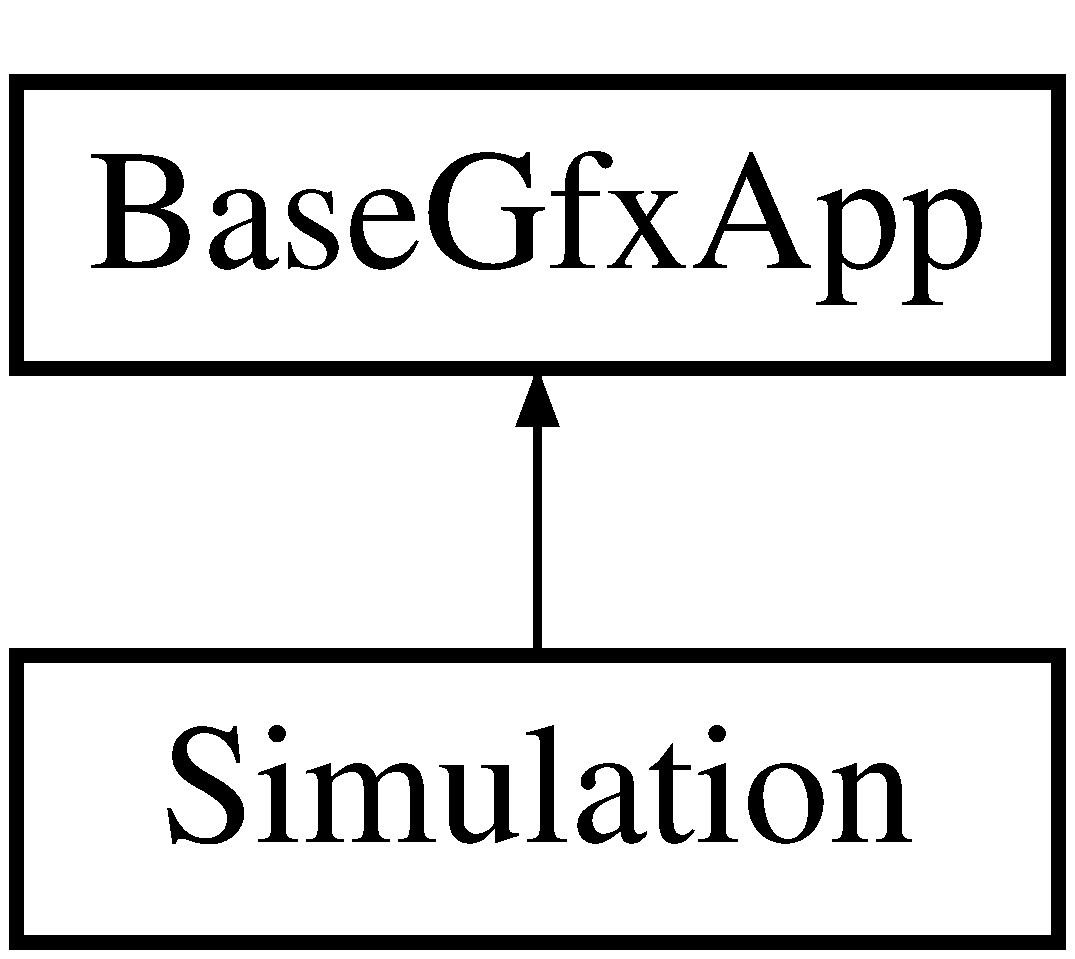
\includegraphics[height=2.000000cm]{classSimulation}
\end{center}
\end{figure}
\subsection*{Public Types}
\begin{DoxyCompactItemize}
\item 
enum {\bfseries U\-I\-Control\-Type} \{ {\bfseries U\-I\-\_\-\-Q\-U\-I\-T} = 0, 
{\bfseries U\-I\-\_\-\-S\-T\-A\-R\-T} = 1, 
{\bfseries U\-I\-\_\-\-P\-A\-U\-S\-E} = 2, 
{\bfseries U\-I\-\_\-\-R\-E\-S\-U\-M\-E} = 3
 \}
\end{DoxyCompactItemize}
\subsection*{Public Member Functions}
\begin{DoxyCompactItemize}
\item 
\hypertarget{classSimulation_a4c669ceaa34c7130966ce45f9de75fbe}{{\bfseries Simulation} (int argc, char $\ast$argv\mbox{[}$\,$\mbox{]}, int width, int height)}\label{classSimulation_a4c669ceaa34c7130966ce45f9de75fbe}

\item 
\hypertarget{classSimulation_a05f768b6836615170f1c43c6c0787fe8}{void {\bfseries update} ()}\label{classSimulation_a05f768b6836615170f1c43c6c0787fe8}

\item 
\hypertarget{classSimulation_a449dcb7d97dfba99efe770de2f399c31}{void {\bfseries display} ()}\label{classSimulation_a449dcb7d97dfba99efe770de2f399c31}

\item 
\hypertarget{classSimulation_a1607cd18e552ab9f4a6f57d362f7121a}{void {\bfseries glui\-Control} (int control\-I\-D)}\label{classSimulation_a1607cd18e552ab9f4a6f57d362f7121a}

\item 
\hypertarget{classSimulation_a786d1ba31d29937f0ac6f3ea88f8a607}{void {\bfseries left\-Mouse\-Down} (int x, int y)}\label{classSimulation_a786d1ba31d29937f0ac6f3ea88f8a607}

\item 
\hypertarget{classSimulation_a62ef254d85017074cd521a5787b5a234}{void {\bfseries left\-Mouse\-Up} (int x, int y)}\label{classSimulation_a62ef254d85017074cd521a5787b5a234}

\item 
void \hyperlink{classSimulation_adaf59b9b5a544f6214d636632a16d6d4}{start} (int)
\item 
void \hyperlink{classSimulation_a72676ce712a367d4124bf88f4165b7b7}{pause} (int)
\item 
void \hyperlink{classSimulation_aecfee72e6cd12d7b2a847a9c9b0634ec}{resume} (int)
\item 
void \hyperlink{classSimulation_ae27c94bdc6071db8dad779b4f0a6ebd9}{quit} (int)
\end{DoxyCompactItemize}
\subsection*{Additional Inherited Members}


\subsection{Detailed Description}
Main application class for the robot simulation. 

\begin{DoxyAuthor}{Author}
C\-Sci3081 Guru
\end{DoxyAuthor}
The \hyperlink{classSimulation}{Simulation} class. This sets up the G\-U\-I and the drawing environment. 

\subsection{Member Function Documentation}
\hypertarget{classSimulation_a72676ce712a367d4124bf88f4165b7b7}{\index{Simulation@{Simulation}!pause@{pause}}
\index{pause@{pause}!Simulation@{Simulation}}
\subsubsection[{pause}]{\setlength{\rightskip}{0pt plus 5cm}void Simulation\-::pause (
\begin{DoxyParamCaption}
\item[{int}]{i}
\end{DoxyParamCaption}
)}}\label{classSimulation_a72676ce712a367d4124bf88f4165b7b7}
Pauses the simulation \hypertarget{classSimulation_ae27c94bdc6071db8dad779b4f0a6ebd9}{\index{Simulation@{Simulation}!quit@{quit}}
\index{quit@{quit}!Simulation@{Simulation}}
\subsubsection[{quit}]{\setlength{\rightskip}{0pt plus 5cm}void Simulation\-::quit (
\begin{DoxyParamCaption}
\item[{int}]{}
\end{DoxyParamCaption}
)}}\label{classSimulation_ae27c94bdc6071db8dad779b4f0a6ebd9}
Quits the simulation \hypertarget{classSimulation_aecfee72e6cd12d7b2a847a9c9b0634ec}{\index{Simulation@{Simulation}!resume@{resume}}
\index{resume@{resume}!Simulation@{Simulation}}
\subsubsection[{resume}]{\setlength{\rightskip}{0pt plus 5cm}void Simulation\-::resume (
\begin{DoxyParamCaption}
\item[{int}]{i}
\end{DoxyParamCaption}
)}}\label{classSimulation_aecfee72e6cd12d7b2a847a9c9b0634ec}
Resumes the simulation \hypertarget{classSimulation_adaf59b9b5a544f6214d636632a16d6d4}{\index{Simulation@{Simulation}!start@{start}}
\index{start@{start}!Simulation@{Simulation}}
\subsubsection[{start}]{\setlength{\rightskip}{0pt plus 5cm}void Simulation\-::start (
\begin{DoxyParamCaption}
\item[{int}]{i}
\end{DoxyParamCaption}
)}}\label{classSimulation_adaf59b9b5a544f6214d636632a16d6d4}
Starts the simulation 

The documentation for this class was generated from the following files\-:\begin{DoxyCompactItemize}
\item 
Simulation.\-h\item 
Simulation.\-cpp\end{DoxyCompactItemize}

\hypertarget{classTarget}{\section{Target Class Reference}
\label{classTarget}\index{Target@{Target}}
}


The class for creating targets.  




{\ttfamily \#include $<$Target.\-h$>$}

Inheritance diagram for Target\-:\begin{figure}[H]
\begin{center}
\leavevmode
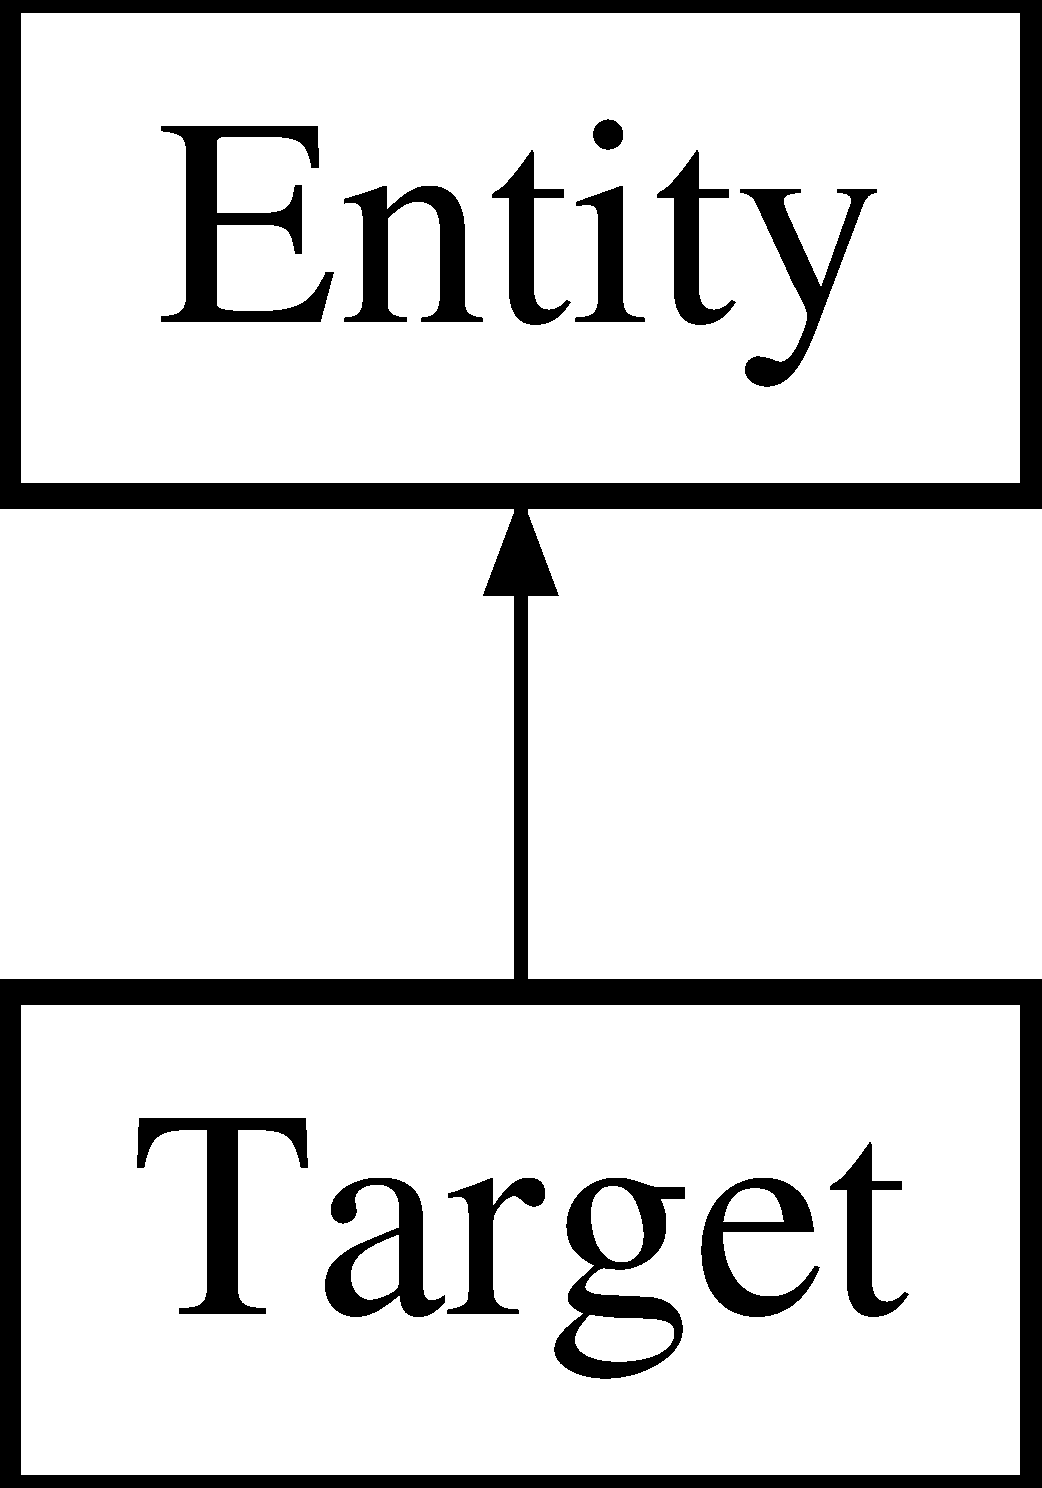
\includegraphics[height=2.000000cm]{classTarget}
\end{center}
\end{figure}
\subsection*{Public Member Functions}
\begin{DoxyCompactItemize}
\item 
\hyperlink{classTarget_ab29ccfc5d42140d4cb1a4ae06bf4aab6}{Target} (int pos\-X, int pos\-Y, int radius)
\item 
\hyperlink{classTarget_a1c253c2c60ff0dd65935c189fd4da1ce}{Target} (\hyperlink{classVector2}{Vector2f} position, int radius)
\item 
void \hyperlink{classTarget_a33e3e447eeba8ded77cb3becf30f98d3}{update} ()
\item 
void \hyperlink{classTarget_a5230b99d26495595cf6879dd6816277a}{render} ()
\end{DoxyCompactItemize}
\subsection*{Additional Inherited Members}


\subsection{Detailed Description}
The class for creating targets. 

\begin{DoxyAuthor}{Author}
Dennis Ehrhardt 

Evan Stuempfig 

Andrew Hartfiel 

David Tran 
\end{DoxyAuthor}


\subsection{Constructor \& Destructor Documentation}
\hypertarget{classTarget_ab29ccfc5d42140d4cb1a4ae06bf4aab6}{\index{Target@{Target}!Target@{Target}}
\index{Target@{Target}!Target@{Target}}
\subsubsection[{Target}]{\setlength{\rightskip}{0pt plus 5cm}Target\-::\-Target (
\begin{DoxyParamCaption}
\item[{int}]{pos\-X, }
\item[{int}]{pos\-Y, }
\item[{int}]{radius}
\end{DoxyParamCaption}
)\hspace{0.3cm}{\ttfamily [inline]}}}\label{classTarget_ab29ccfc5d42140d4cb1a4ae06bf4aab6}
This constructor requires three parameters\-: x position, y position, and radius. 
\begin{DoxyParams}{Parameters}
{\em pos\-X} & the x position in pixels \\
\hline
{\em pos\-Y} & the y position in pixels \\
\hline
{\em radius} & the radius in pixels \\
\hline
\end{DoxyParams}
\hypertarget{classTarget_a1c253c2c60ff0dd65935c189fd4da1ce}{\index{Target@{Target}!Target@{Target}}
\index{Target@{Target}!Target@{Target}}
\subsubsection[{Target}]{\setlength{\rightskip}{0pt plus 5cm}Target\-::\-Target (
\begin{DoxyParamCaption}
\item[{{\bf Vector2f}}]{position, }
\item[{int}]{radius}
\end{DoxyParamCaption}
)\hspace{0.3cm}{\ttfamily [inline]}}}\label{classTarget_a1c253c2c60ff0dd65935c189fd4da1ce}
This constructor requires two parameters\-: location and radius. 
\begin{DoxyParams}{Parameters}
{\em location} & the x and y position in pixels as a \hyperlink{classVector2}{Vector2} \\
\hline
{\em radius} & the radius in pixels \\
\hline
\end{DoxyParams}


\subsection{Member Function Documentation}
\hypertarget{classTarget_a5230b99d26495595cf6879dd6816277a}{\index{Target@{Target}!render@{render}}
\index{render@{render}!Target@{Target}}
\subsubsection[{render}]{\setlength{\rightskip}{0pt plus 5cm}void Target\-::render (
\begin{DoxyParamCaption}
{}
\end{DoxyParamCaption}
)\hspace{0.3cm}{\ttfamily [virtual]}}}\label{classTarget_a5230b99d26495595cf6879dd6816277a}
Draw the target on the screen 

Reimplemented from \hyperlink{classEntity_af5ca41372ff108e4c044e8d927995a27}{Entity}.

\hypertarget{classTarget_a33e3e447eeba8ded77cb3becf30f98d3}{\index{Target@{Target}!update@{update}}
\index{update@{update}!Target@{Target}}
\subsubsection[{update}]{\setlength{\rightskip}{0pt plus 5cm}void Target\-::update (
\begin{DoxyParamCaption}
{}
\end{DoxyParamCaption}
)\hspace{0.3cm}{\ttfamily [virtual]}}}\label{classTarget_a33e3e447eeba8ded77cb3becf30f98d3}
Update the target's position and behavior 

Reimplemented from \hyperlink{classEntity_a00b6eeaf99b35c8f8b10b5fbfc1baf4f}{Entity}.



The documentation for this class was generated from the following files\-:\begin{DoxyCompactItemize}
\item 
Entity/Target.\-h\item 
Entity/Target.\-cpp\end{DoxyCompactItemize}

\hypertarget{classVector2}{\section{Vector2$<$ T $>$ Class Template Reference}
\label{classVector2}\index{Vector2$<$ T $>$@{Vector2$<$ T $>$}}
}


A two dimensional templated vector of the form (x, y)  




{\ttfamily \#include $<$Vector2.\-h$>$}

\subsection*{Public Member Functions}
\begin{DoxyCompactItemize}
\item 
\hyperlink{classVector2_ae2f1223cb0d664aa73afb789086a4174}{Vector2} ()
\item 
\hyperlink{classVector2_ad79ae2f328cd2b8d895566305acdf04d}{Vector2} (T xcoord, T ycoord)
\item 
bool \hyperlink{classVector2_a84cd3fd4795023c476c544c4d889faf1}{operator==} (\hyperlink{classVector2}{Vector2}$<$ T $>$ const \&)
\item 
bool \hyperlink{classVector2_a665455a989653e79f21b03302619d6bd}{operator!=} (\hyperlink{classVector2}{Vector2}$<$ T $>$ const \&)
\item 
\hyperlink{classVector2}{Vector2}$<$ T $>$ \hyperlink{classVector2_a6434426c127577c1f66525bb903aec52}{operator=} (\hyperlink{classVector2}{Vector2}$<$ T $>$ const \&)
\item 
\hyperlink{classVector2}{Vector2}$<$ T $>$ \hyperlink{classVector2_aa581ba273bb347e93058a2e2b696a329}{set\-Values} (T x, T y)
\item 
\hyperlink{classVector2}{Vector2} \hyperlink{classVector2_af2b0a7852790bdf522f74db750b6d143}{zero} ()
\item 
\hyperlink{classVector2}{Vector2}$<$ T $>$ \hyperlink{classVector2_a98ffd6c779d7a4011f6a8f1a05ee6f9a}{operator+} (\hyperlink{classVector2}{Vector2}$<$ T $>$ const \&) const 
\item 
\hyperlink{classVector2}{Vector2}$<$ T $>$ \hyperlink{classVector2_ada9ee9f6d6c88e6e8c7a9c84da177b49}{operator+=} (\hyperlink{classVector2}{Vector2}$<$ T $>$ const \&)
\item 
\hyperlink{classVector2}{Vector2}$<$ T $>$ \hyperlink{classVector2_a43088957bb9fba96a73d564ca7c68fb6}{operator-\/} (\hyperlink{classVector2}{Vector2}$<$ T $>$ const \&) const 
\item 
\hyperlink{classVector2}{Vector2}$<$ T $>$ \hyperlink{classVector2_adf7a38a9d43c6830708057c30ddbf5f9}{operator-\/=} (\hyperlink{classVector2}{Vector2}$<$ T $>$ const \&)
\item 
\hyperlink{classVector2}{Vector2}$<$ T $>$ \hyperlink{classVector2_ad630c141ea4b5c348d1dbe90fd16af95}{operator$\ast$} (T) const 
\item 
\hyperlink{classVector2}{Vector2}$<$ T $>$ \hyperlink{classVector2_aff6f9727727cb72c696ae8408ee3175f}{operator$\ast$=} (T const \&)
\item 
float \hyperlink{classVector2_a9d13fbfc940b88cf117b90c7bcffeec5}{dot} (\hyperlink{classVector2}{Vector2}$<$ T $>$ const \&v) const 
\item 
float \hyperlink{classVector2_ada039a01838e14cf97b2f995f4748a61}{zcross} (\hyperlink{classVector2}{Vector2}$<$ T $>$ const \&v) const 
\item 
float \hyperlink{classVector2_a2ba2726deca326f6cf6f90cf96c6417b}{magnitude} () const 
\item 
float \hyperlink{classVector2_aca33fd3614fba0f29f6145642085879f}{magnitude\-Squared} () const 
\item 
float \hyperlink{classVector2_aa4deaff6744e5c52980c9543cde879c2}{length} (\hyperlink{classVector2}{Vector2}$<$ T $>$ vec) const 
\item 
float \hyperlink{classVector2_a6d33069838bf0cf4f068da4cc5d1784e}{length\-Squared} (\hyperlink{classVector2}{Vector2}$<$ T $>$ vec) const 
\item 
\hyperlink{classVector2}{Vector2} \hyperlink{classVector2_a8e5a913965bcd2725ca0960022874dcc}{normalize} ()
\item 
\hyperlink{classVector2}{Vector2} \hyperlink{classVector2_ad3ad9070482b89306e14e6cb127e1205}{clamp} (T max)
\item 
\hyperlink{classVector2}{Vector2} \hyperlink{classVector2_a3c6020b1331c100a2412f254fcdd44df}{clamp\-X} (T max)
\item 
\hyperlink{classVector2}{Vector2} \hyperlink{classVector2_a6cc7835e6bc56dd0fee04083640ff4b6}{clamp\-Y} (T max)
\item 
\hyperlink{classVector2}{Vector2} \hyperlink{classVector2_af02626f147b83492346921bfb44adeb4}{rotate} (float)
\item 
float \hyperlink{classVector2_a820da4470e33691b242bd69b162014b4}{angle} (\hyperlink{classVector2}{Vector2}$<$ T $>$ const \&v) const 
\item 
float \hyperlink{classVector2_aa481cb08d305491d9e3581946c94ceb4}{angle\-Magnitude} (\hyperlink{classVector2}{Vector2}$<$ T $>$ const \&v) const 
\item 
\hyperlink{classVector2}{Vector2}$<$ T $>$ \hyperlink{classVector2_a3447a814a110582b4c8b9944ce0d299e}{flip} ()
\end{DoxyCompactItemize}
\subsection*{Public Attributes}
\begin{DoxyCompactItemize}
\item 
\hypertarget{classVector2_a78fa1f2ed5e261c7fbeb8f3536a1ee34}{T {\bfseries x}}\label{classVector2_a78fa1f2ed5e261c7fbeb8f3536a1ee34}

\item 
\hypertarget{classVector2_a6cfed8355591aa269f4dba43bd806ef9}{T {\bfseries y}}\label{classVector2_a6cfed8355591aa269f4dba43bd806ef9}

\end{DoxyCompactItemize}


\subsection{Detailed Description}
\subsubsection*{template$<$class T$>$class Vector2$<$ T $>$}

A two dimensional templated vector of the form (x, y) 

\begin{DoxyAuthor}{Author}
Dennis Ehrhardt 
\end{DoxyAuthor}


\subsection{Constructor \& Destructor Documentation}
\hypertarget{classVector2_ae2f1223cb0d664aa73afb789086a4174}{\index{Vector2@{Vector2}!Vector2@{Vector2}}
\index{Vector2@{Vector2}!Vector2@{Vector2}}
\subsubsection[{Vector2}]{\setlength{\rightskip}{0pt plus 5cm}template$<$class T$>$ {\bf Vector2}$<$ T $>$\-::{\bf Vector2} (
\begin{DoxyParamCaption}
{}
\end{DoxyParamCaption}
)\hspace{0.3cm}{\ttfamily [inline]}}}\label{classVector2_ae2f1223cb0d664aa73afb789086a4174}
The default constructor creates a zero vector. \hypertarget{classVector2_ad79ae2f328cd2b8d895566305acdf04d}{\index{Vector2@{Vector2}!Vector2@{Vector2}}
\index{Vector2@{Vector2}!Vector2@{Vector2}}
\subsubsection[{Vector2}]{\setlength{\rightskip}{0pt plus 5cm}template$<$class T$>$ {\bf Vector2}$<$ T $>$\-::{\bf Vector2} (
\begin{DoxyParamCaption}
\item[{T}]{xcoord, }
\item[{T}]{ycoord}
\end{DoxyParamCaption}
)\hspace{0.3cm}{\ttfamily [inline]}}}\label{classVector2_ad79ae2f328cd2b8d895566305acdf04d}
This constructor requires two parameters\-: xcoord and ycoord. 
\begin{DoxyParams}{Parameters}
{\em xcoord} & the x coordinate in pixels \\
\hline
{\em pos\-Y} & the y coordinate in pixels \\
\hline
\end{DoxyParams}


\subsection{Member Function Documentation}
\hypertarget{classVector2_a820da4470e33691b242bd69b162014b4}{\index{Vector2@{Vector2}!angle@{angle}}
\index{angle@{angle}!Vector2@{Vector2}}
\subsubsection[{angle}]{\setlength{\rightskip}{0pt plus 5cm}template$<$class T$>$ float {\bf Vector2}$<$ T $>$\-::angle (
\begin{DoxyParamCaption}
\item[{{\bf Vector2}$<$ T $>$ const \&}]{v}
\end{DoxyParamCaption}
) const}}\label{classVector2_a820da4470e33691b242bd69b162014b4}
Returns the angle between two vectors 
\begin{DoxyParams}{Parameters}
{\em v} & the second vector \\
\hline
\end{DoxyParams}
\begin{DoxyReturn}{Returns}
the angle betweem two vectors from -\/\-P\-I to P\-I 
\end{DoxyReturn}
\hypertarget{classVector2_aa481cb08d305491d9e3581946c94ceb4}{\index{Vector2@{Vector2}!angle\-Magnitude@{angle\-Magnitude}}
\index{angle\-Magnitude@{angle\-Magnitude}!Vector2@{Vector2}}
\subsubsection[{angle\-Magnitude}]{\setlength{\rightskip}{0pt plus 5cm}template$<$class T$>$ float {\bf Vector2}$<$ T $>$\-::angle\-Magnitude (
\begin{DoxyParamCaption}
\item[{{\bf Vector2}$<$ T $>$ const \&}]{v}
\end{DoxyParamCaption}
) const}}\label{classVector2_aa481cb08d305491d9e3581946c94ceb4}
Returns the magnitude of angle between two vectors 
\begin{DoxyParams}{Parameters}
{\em v} & the second vector \\
\hline
\end{DoxyParams}
\begin{DoxyReturn}{Returns}
the angle betweem two vectors from 0 to P\-I 
\end{DoxyReturn}
\hypertarget{classVector2_ad3ad9070482b89306e14e6cb127e1205}{\index{Vector2@{Vector2}!clamp@{clamp}}
\index{clamp@{clamp}!Vector2@{Vector2}}
\subsubsection[{clamp}]{\setlength{\rightskip}{0pt plus 5cm}template$<$class T$>$ {\bf Vector2}$<$ T $>$ {\bf Vector2}$<$ T $>$\-::clamp (
\begin{DoxyParamCaption}
\item[{T}]{max}
\end{DoxyParamCaption}
)}}\label{classVector2_ad3ad9070482b89306e14e6cb127e1205}
Clamps the vector to a maximum magnitude 
\begin{DoxyParams}{Parameters}
{\em max} & the maximum value \\
\hline
\end{DoxyParams}
\begin{DoxyReturn}{Returns}
The clamped vector (\hyperlink{classVector2}{Vector2}) 
\end{DoxyReturn}
\hypertarget{classVector2_a3c6020b1331c100a2412f254fcdd44df}{\index{Vector2@{Vector2}!clamp\-X@{clamp\-X}}
\index{clamp\-X@{clamp\-X}!Vector2@{Vector2}}
\subsubsection[{clamp\-X}]{\setlength{\rightskip}{0pt plus 5cm}template$<$class T$>$ {\bf Vector2}$<$ T $>$ {\bf Vector2}$<$ T $>$\-::clamp\-X (
\begin{DoxyParamCaption}
\item[{T}]{max}
\end{DoxyParamCaption}
)}}\label{classVector2_a3c6020b1331c100a2412f254fcdd44df}
Clamps the x component of the vector to a maximum 
\begin{DoxyParams}{Parameters}
{\em max} & the maximum value \\
\hline
\end{DoxyParams}
\begin{DoxyReturn}{Returns}
The clamped vector (\hyperlink{classVector2}{Vector2}) 
\end{DoxyReturn}
\hypertarget{classVector2_a6cc7835e6bc56dd0fee04083640ff4b6}{\index{Vector2@{Vector2}!clamp\-Y@{clamp\-Y}}
\index{clamp\-Y@{clamp\-Y}!Vector2@{Vector2}}
\subsubsection[{clamp\-Y}]{\setlength{\rightskip}{0pt plus 5cm}template$<$class T$>$ {\bf Vector2}$<$ T $>$ {\bf Vector2}$<$ T $>$\-::clamp\-Y (
\begin{DoxyParamCaption}
\item[{T}]{max}
\end{DoxyParamCaption}
)}}\label{classVector2_a6cc7835e6bc56dd0fee04083640ff4b6}
Clamps the y component of the vector to a maximum 
\begin{DoxyParams}{Parameters}
{\em max} & the maximum value \\
\hline
\end{DoxyParams}
\begin{DoxyReturn}{Returns}
The clamped vector (\hyperlink{classVector2}{Vector2}) 
\end{DoxyReturn}
\hypertarget{classVector2_a9d13fbfc940b88cf117b90c7bcffeec5}{\index{Vector2@{Vector2}!dot@{dot}}
\index{dot@{dot}!Vector2@{Vector2}}
\subsubsection[{dot}]{\setlength{\rightskip}{0pt plus 5cm}template$<$class T$>$ float {\bf Vector2}$<$ T $>$\-::dot (
\begin{DoxyParamCaption}
\item[{{\bf Vector2}$<$ T $>$ const \&}]{v}
\end{DoxyParamCaption}
) const}}\label{classVector2_a9d13fbfc940b88cf117b90c7bcffeec5}
Returns the dot product of this dot v 
\begin{DoxyParams}{Parameters}
{\em v} & the second vector \\
\hline
\end{DoxyParams}
\begin{DoxyReturn}{Returns}
The dot product (float) 
\end{DoxyReturn}
\hypertarget{classVector2_a3447a814a110582b4c8b9944ce0d299e}{\index{Vector2@{Vector2}!flip@{flip}}
\index{flip@{flip}!Vector2@{Vector2}}
\subsubsection[{flip}]{\setlength{\rightskip}{0pt plus 5cm}template$<$class T $>$ {\bf Vector2}$<$ T $>$ {\bf Vector2}$<$ T $>$\-::flip (
\begin{DoxyParamCaption}
{}
\end{DoxyParamCaption}
)}}\label{classVector2_a3447a814a110582b4c8b9944ce0d299e}
Rotates the vector by pi radians \begin{DoxyReturn}{Returns}
The flipped vector (\hyperlink{classVector2}{Vector2}) 
\end{DoxyReturn}
\hypertarget{classVector2_aa4deaff6744e5c52980c9543cde879c2}{\index{Vector2@{Vector2}!length@{length}}
\index{length@{length}!Vector2@{Vector2}}
\subsubsection[{length}]{\setlength{\rightskip}{0pt plus 5cm}template$<$class T$>$ float {\bf Vector2}$<$ T $>$\-::length (
\begin{DoxyParamCaption}
\item[{{\bf Vector2}$<$ T $>$}]{vec}
\end{DoxyParamCaption}
) const}}\label{classVector2_aa4deaff6744e5c52980c9543cde879c2}
Returns the distance between two vectors 
\begin{DoxyParams}{Parameters}
{\em vec} & the second vector \\
\hline
\end{DoxyParams}
\begin{DoxyReturn}{Returns}
The distance between the vectors as a (float) 
\end{DoxyReturn}
\hypertarget{classVector2_a6d33069838bf0cf4f068da4cc5d1784e}{\index{Vector2@{Vector2}!length\-Squared@{length\-Squared}}
\index{length\-Squared@{length\-Squared}!Vector2@{Vector2}}
\subsubsection[{length\-Squared}]{\setlength{\rightskip}{0pt plus 5cm}template$<$class T$>$ float {\bf Vector2}$<$ T $>$\-::length\-Squared (
\begin{DoxyParamCaption}
\item[{{\bf Vector2}$<$ T $>$}]{vec}
\end{DoxyParamCaption}
) const}}\label{classVector2_a6d33069838bf0cf4f068da4cc5d1784e}
Returns the distance squared between two vectors 
\begin{DoxyParams}{Parameters}
{\em vec} & the second vector \\
\hline
\end{DoxyParams}
\begin{DoxyReturn}{Returns}
The distance between the vectors squared (float) 
\end{DoxyReturn}
\hypertarget{classVector2_a2ba2726deca326f6cf6f90cf96c6417b}{\index{Vector2@{Vector2}!magnitude@{magnitude}}
\index{magnitude@{magnitude}!Vector2@{Vector2}}
\subsubsection[{magnitude}]{\setlength{\rightskip}{0pt plus 5cm}template$<$class T $>$ float {\bf Vector2}$<$ T $>$\-::magnitude (
\begin{DoxyParamCaption}
{}
\end{DoxyParamCaption}
) const}}\label{classVector2_a2ba2726deca326f6cf6f90cf96c6417b}
Returns the magnitude of the vector \begin{DoxyReturn}{Returns}
Magnitude (float) 
\end{DoxyReturn}
\hypertarget{classVector2_aca33fd3614fba0f29f6145642085879f}{\index{Vector2@{Vector2}!magnitude\-Squared@{magnitude\-Squared}}
\index{magnitude\-Squared@{magnitude\-Squared}!Vector2@{Vector2}}
\subsubsection[{magnitude\-Squared}]{\setlength{\rightskip}{0pt plus 5cm}template$<$class T $>$ float {\bf Vector2}$<$ T $>$\-::magnitude\-Squared (
\begin{DoxyParamCaption}
{}
\end{DoxyParamCaption}
) const}}\label{classVector2_aca33fd3614fba0f29f6145642085879f}
Returns the magnitude squared of the vector \begin{DoxyReturn}{Returns}
Magnitude squared (float) 
\end{DoxyReturn}
\hypertarget{classVector2_a8e5a913965bcd2725ca0960022874dcc}{\index{Vector2@{Vector2}!normalize@{normalize}}
\index{normalize@{normalize}!Vector2@{Vector2}}
\subsubsection[{normalize}]{\setlength{\rightskip}{0pt plus 5cm}template$<$class T $>$ {\bf Vector2}$<$ T $>$ {\bf Vector2}$<$ T $>$\-::normalize (
\begin{DoxyParamCaption}
{}
\end{DoxyParamCaption}
)}}\label{classVector2_a8e5a913965bcd2725ca0960022874dcc}
Makes the vector have a magnitude of 1 \begin{DoxyReturn}{Returns}
The normalized vector (\hyperlink{classVector2}{Vector2}) 
\end{DoxyReturn}
\hypertarget{classVector2_a665455a989653e79f21b03302619d6bd}{\index{Vector2@{Vector2}!operator!=@{operator!=}}
\index{operator!=@{operator!=}!Vector2@{Vector2}}
\subsubsection[{operator!=}]{\setlength{\rightskip}{0pt plus 5cm}template$<$class T$>$ bool {\bf Vector2}$<$ T $>$\-::operator!= (
\begin{DoxyParamCaption}
\item[{{\bf Vector2}$<$ T $>$ const \&}]{vec}
\end{DoxyParamCaption}
)\hspace{0.3cm}{\ttfamily [inline]}}}\label{classVector2_a665455a989653e79f21b03302619d6bd}
Override != operator to correctly check if vectors are not equivalent \hypertarget{classVector2_ad630c141ea4b5c348d1dbe90fd16af95}{\index{Vector2@{Vector2}!operator$\ast$@{operator$\ast$}}
\index{operator$\ast$@{operator$\ast$}!Vector2@{Vector2}}
\subsubsection[{operator$\ast$}]{\setlength{\rightskip}{0pt plus 5cm}template$<$class T$>$ {\bf Vector2}$<$ T $>$ {\bf Vector2}$<$ T $>$\-::operator$\ast$ (
\begin{DoxyParamCaption}
\item[{T}]{scalar}
\end{DoxyParamCaption}
) const}}\label{classVector2_ad630c141ea4b5c348d1dbe90fd16af95}
Override $\ast$ operator to multiply the vector by a scalar \begin{DoxyReturn}{Returns}
The resulting vector (\hyperlink{classVector2}{Vector2}) 
\end{DoxyReturn}
\hypertarget{classVector2_aff6f9727727cb72c696ae8408ee3175f}{\index{Vector2@{Vector2}!operator$\ast$=@{operator$\ast$=}}
\index{operator$\ast$=@{operator$\ast$=}!Vector2@{Vector2}}
\subsubsection[{operator$\ast$=}]{\setlength{\rightskip}{0pt plus 5cm}template$<$class T$>$ {\bf Vector2}$<$ T $>$ {\bf Vector2}$<$ T $>$\-::operator$\ast$= (
\begin{DoxyParamCaption}
\item[{T const \&}]{scalar}
\end{DoxyParamCaption}
)}}\label{classVector2_aff6f9727727cb72c696ae8408ee3175f}
Override $\ast$= operator to multiply the vector by a scalar and set to the result \begin{DoxyReturn}{Returns}
The resulting vector (\hyperlink{classVector2}{Vector2}) 
\end{DoxyReturn}
\hypertarget{classVector2_a98ffd6c779d7a4011f6a8f1a05ee6f9a}{\index{Vector2@{Vector2}!operator+@{operator+}}
\index{operator+@{operator+}!Vector2@{Vector2}}
\subsubsection[{operator+}]{\setlength{\rightskip}{0pt plus 5cm}template$<$class T$>$ {\bf Vector2}$<$ T $>$ {\bf Vector2}$<$ T $>$\-::operator+ (
\begin{DoxyParamCaption}
\item[{{\bf Vector2}$<$ T $>$ const \&}]{v}
\end{DoxyParamCaption}
) const}}\label{classVector2_a98ffd6c779d7a4011f6a8f1a05ee6f9a}
Override + operator to correctly add another vector \begin{DoxyReturn}{Returns}
The resulting vector (\hyperlink{classVector2}{Vector2}) 
\end{DoxyReturn}
\hypertarget{classVector2_ada9ee9f6d6c88e6e8c7a9c84da177b49}{\index{Vector2@{Vector2}!operator+=@{operator+=}}
\index{operator+=@{operator+=}!Vector2@{Vector2}}
\subsubsection[{operator+=}]{\setlength{\rightskip}{0pt plus 5cm}template$<$class T$>$ {\bf Vector2}$<$ T $>$ {\bf Vector2}$<$ T $>$\-::operator+= (
\begin{DoxyParamCaption}
\item[{{\bf Vector2}$<$ T $>$ const \&}]{v}
\end{DoxyParamCaption}
)}}\label{classVector2_ada9ee9f6d6c88e6e8c7a9c84da177b49}
Override += operator to add another vector and set to the result \begin{DoxyReturn}{Returns}
The resulting vector (\hyperlink{classVector2}{Vector2}) 
\end{DoxyReturn}
\hypertarget{classVector2_a43088957bb9fba96a73d564ca7c68fb6}{\index{Vector2@{Vector2}!operator-\/@{operator-\/}}
\index{operator-\/@{operator-\/}!Vector2@{Vector2}}
\subsubsection[{operator-\/}]{\setlength{\rightskip}{0pt plus 5cm}template$<$class T$>$ {\bf Vector2}$<$ T $>$ {\bf Vector2}$<$ T $>$\-::operator-\/ (
\begin{DoxyParamCaption}
\item[{{\bf Vector2}$<$ T $>$ const \&}]{v}
\end{DoxyParamCaption}
) const}}\label{classVector2_a43088957bb9fba96a73d564ca7c68fb6}
Override -\/ operator to correctly subtract another vector \begin{DoxyReturn}{Returns}
The resulting vector (\hyperlink{classVector2}{Vector2}) 
\end{DoxyReturn}
\hypertarget{classVector2_adf7a38a9d43c6830708057c30ddbf5f9}{\index{Vector2@{Vector2}!operator-\/=@{operator-\/=}}
\index{operator-\/=@{operator-\/=}!Vector2@{Vector2}}
\subsubsection[{operator-\/=}]{\setlength{\rightskip}{0pt plus 5cm}template$<$class T$>$ {\bf Vector2}$<$ T $>$ {\bf Vector2}$<$ T $>$\-::operator-\/= (
\begin{DoxyParamCaption}
\item[{{\bf Vector2}$<$ T $>$ const \&}]{v}
\end{DoxyParamCaption}
)}}\label{classVector2_adf7a38a9d43c6830708057c30ddbf5f9}
Override -\/= operator to subtract another vector and set to the result \begin{DoxyReturn}{Returns}
The resulting vector (\hyperlink{classVector2}{Vector2}) 
\end{DoxyReturn}
\hypertarget{classVector2_a6434426c127577c1f66525bb903aec52}{\index{Vector2@{Vector2}!operator=@{operator=}}
\index{operator=@{operator=}!Vector2@{Vector2}}
\subsubsection[{operator=}]{\setlength{\rightskip}{0pt plus 5cm}template$<$class T$>$ {\bf Vector2}$<$ T $>$ {\bf Vector2}$<$ T $>$\-::operator= (
\begin{DoxyParamCaption}
\item[{{\bf Vector2}$<$ T $>$ const \&}]{v}
\end{DoxyParamCaption}
)}}\label{classVector2_a6434426c127577c1f66525bb903aec52}
Override = operator to set a vector equal to another \hypertarget{classVector2_a84cd3fd4795023c476c544c4d889faf1}{\index{Vector2@{Vector2}!operator==@{operator==}}
\index{operator==@{operator==}!Vector2@{Vector2}}
\subsubsection[{operator==}]{\setlength{\rightskip}{0pt plus 5cm}template$<$class T$>$ bool {\bf Vector2}$<$ T $>$\-::operator== (
\begin{DoxyParamCaption}
\item[{{\bf Vector2}$<$ T $>$ const \&}]{vec}
\end{DoxyParamCaption}
)\hspace{0.3cm}{\ttfamily [inline]}}}\label{classVector2_a84cd3fd4795023c476c544c4d889faf1}
Override == operator to correctly check if vectors are equivalent \hypertarget{classVector2_af02626f147b83492346921bfb44adeb4}{\index{Vector2@{Vector2}!rotate@{rotate}}
\index{rotate@{rotate}!Vector2@{Vector2}}
\subsubsection[{rotate}]{\setlength{\rightskip}{0pt plus 5cm}template$<$class T $>$ {\bf Vector2}$<$ T $>$ {\bf Vector2}$<$ T $>$\-::rotate (
\begin{DoxyParamCaption}
\item[{float}]{angle}
\end{DoxyParamCaption}
)}}\label{classVector2_af02626f147b83492346921bfb44adeb4}
Rotates the Vector in radians 
\begin{DoxyParams}{Parameters}
{\em angle} & angle in radians \\
\hline
\end{DoxyParams}
\begin{DoxyReturn}{Returns}
The rotated vector (\hyperlink{classVector2}{Vector2}) 
\end{DoxyReturn}
\hypertarget{classVector2_aa581ba273bb347e93058a2e2b696a329}{\index{Vector2@{Vector2}!set\-Values@{set\-Values}}
\index{set\-Values@{set\-Values}!Vector2@{Vector2}}
\subsubsection[{set\-Values}]{\setlength{\rightskip}{0pt plus 5cm}template$<$class T$>$ {\bf Vector2}$<$ T $>$ {\bf Vector2}$<$ T $>$\-::set\-Values (
\begin{DoxyParamCaption}
\item[{T}]{x, }
\item[{T}]{y}
\end{DoxyParamCaption}
)}}\label{classVector2_aa581ba273bb347e93058a2e2b696a329}
Set x and y of the vector 
\begin{DoxyParams}{Parameters}
{\em x} & the x value \\
\hline
{\em y} & the y value \\
\hline
\end{DoxyParams}
\begin{DoxyReturn}{Returns}
The new vector (\hyperlink{classVector2}{Vector2}) 
\end{DoxyReturn}
\hypertarget{classVector2_ada039a01838e14cf97b2f995f4748a61}{\index{Vector2@{Vector2}!zcross@{zcross}}
\index{zcross@{zcross}!Vector2@{Vector2}}
\subsubsection[{zcross}]{\setlength{\rightskip}{0pt plus 5cm}template$<$class T$>$ float {\bf Vector2}$<$ T $>$\-::zcross (
\begin{DoxyParamCaption}
\item[{{\bf Vector2}$<$ T $>$ const \&}]{v}
\end{DoxyParamCaption}
) const}}\label{classVector2_ada039a01838e14cf97b2f995f4748a61}
Computes the zcross product between this and vector v 
\begin{DoxyParams}{Parameters}
{\em v} & the second vector \\
\hline
\end{DoxyParams}
\begin{DoxyReturn}{Returns}
The z component of the zcross product 
\end{DoxyReturn}
\hypertarget{classVector2_af2b0a7852790bdf522f74db750b6d143}{\index{Vector2@{Vector2}!zero@{zero}}
\index{zero@{zero}!Vector2@{Vector2}}
\subsubsection[{zero}]{\setlength{\rightskip}{0pt plus 5cm}template$<$class T $>$ {\bf Vector2}$<$ T $>$ {\bf Vector2}$<$ T $>$\-::zero (
\begin{DoxyParamCaption}
{}
\end{DoxyParamCaption}
)}}\label{classVector2_af2b0a7852790bdf522f74db750b6d143}
Sets the Vector to (0,0) \begin{DoxyReturn}{Returns}
The vector (0,0) (\hyperlink{classVector2}{Vector2}) 
\end{DoxyReturn}


The documentation for this class was generated from the following files\-:\begin{DoxyCompactItemize}
\item 
Vector2.\-h\item 
Vector2.\-cpp\end{DoxyCompactItemize}

\chapter{File Documentation}
\hypertarget{BaseGfxApp_8h}{\section{Base\-Gfx\-App.\-h File Reference}
\label{BaseGfxApp_8h}\index{Base\-Gfx\-App.\-h@{Base\-Gfx\-App.\-h}}
}


The basic application class for C\-Sci-\/3081 project. Uses G\-L\-U\-T and G\-L\-U\-I and wraps them in a nice C++ interface.  


{\ttfamily \#include $<$string$>$}\\*
{\ttfamily \#include $<$iostream$>$}\\*
{\ttfamily \#include $<$assert.\-h$>$}\\*
{\ttfamily \#include $<$G\-L/glui.\-h$>$}\\*
\subsection*{Classes}
\begin{DoxyCompactItemize}
\item 
class \hyperlink{classBaseGfxApp}{Base\-Gfx\-App}
\end{DoxyCompactItemize}


\subsection{Detailed Description}
The basic application class for C\-Sci-\/3081 project. Uses G\-L\-U\-T and G\-L\-U\-I and wraps them in a nice C++ interface. \begin{DoxyAuthor}{Author}
C\-Sci3081 Guru 
\end{DoxyAuthor}

\hypertarget{main_8cpp}{\section{main.\-cpp File Reference}
\label{main_8cpp}\index{main.\-cpp@{main.\-cpp}}
}


Main function.  


{\ttfamily \#include \char`\"{}Simulation.\-h\char`\"{}}\\*
\subsection*{Functions}
\begin{DoxyCompactItemize}
\item 
\hypertarget{main_8cpp_a0ddf1224851353fc92bfbff6f499fa97}{int {\bfseries main} (int argc, char $\ast$argv\mbox{[}$\,$\mbox{]})}\label{main_8cpp_a0ddf1224851353fc92bfbff6f499fa97}

\end{DoxyCompactItemize}


\subsection{Detailed Description}
Main function. \begin{DoxyAuthor}{Author}
C\-Sci5107 Guru 
\end{DoxyAuthor}

%--- End generated contents ---

% Index
\newpage
\phantomsection
\addcontentsline{toc}{chapter}{Index}
\printindex

\end{document}
